\documentclass[aspectratio=169,]{beamer}

% -------------------------------------------------------------------------
% 1. REQUIRED PACKAGES (The "Batteries" Quarto usually includes)
% -------------------------------------------------------------------------
\usepackage{graphicx}
\usepackage{booktabs}
\usepackage{longtable}
\usepackage{hyperref}
\usepackage{array}      % <--- ADD THIS LINE HERE
\usepackage[most]{tcolorbox} % REQUIRED for Quarto Callouts
\usepackage{fontawesome5}    % REQUIRED for Callout Icons
\usepackage{framed}          % REQUIRED for standard blocks
\usepackage{tikz}
\usetikzlibrary{arrows.meta}

% Fix for Pandoc's "tightlist"
\providecommand{\tightlist}{%
  \setlength{\itemsep}{0pt}\setlength{\parskip}{0pt}}

% -------------------------------------------------------------------------
% 2. CUSTOM DESIGN PACKAGES
% -------------------------------------------------------------------------
\usepackage{tikz}
\usepackage{calc}
\usepackage{xcolor}
\usepackage{xparse} 
\usepackage{etoolbox} 
\usepackage[default]{sourcesanspro} 
\usetikzlibrary{calc, positioning, shapes.geometric}

% -------------------------------------------------------------------------
% DEFINE QUARTO CALLOUT COLORS (REQUIRED)
% -------------------------------------------------------------------------
% We map these to your "Elegant Dark Mode" aesthetic.
% Note: Quarto expects these EXACT names.

% 1. Note (Blue)
\definecolor{quarto-callout-note-color}{HTML}{3498DB}        % Icon/Title Color
\definecolor{quarto-callout-note-color-frame}{HTML}{2980B9}  % Border Color

% 2. Tip (Green)
\definecolor{quarto-callout-tip-color}{HTML}{27AE60}
\definecolor{quarto-callout-tip-color-frame}{HTML}{2ECC71}

% 3. Important (Red/Crimson)
\definecolor{quarto-callout-important-color}{HTML}{C0392B}
\definecolor{quarto-callout-important-color-frame}{HTML}{E74C3C}

% 4. Warning (Orange)
\definecolor{quarto-callout-warning-color}{HTML}{F39C12}
\definecolor{quarto-callout-warning-color-frame}{HTML}{E67E22}

% 5. Caution (Yellow/Gold)
\definecolor{quarto-callout-caution-color}{HTML}{F1C40F}
\definecolor{quarto-callout-caution-color-frame}{HTML}{D4AC0D}

% Add this right before \begin{document}
\newcommand{\Est}[1]{\textcolor{quarto-callout-important-color}{\mathbf{#1}}}


% -------------------------------------------------------------------------
% NEW: COLOR THEME COMMANDS (Robust Single-Slide Overrides)
% -------------------------------------------------------------------------

% 1. Light Mode Command
\newcommand{\LightMode}{
  % 1. Draw White Background (TikZ Overlay)
  \begin{tikzpicture}[remember picture, overlay]
    \fill[white] (current page.south west) rectangle (current page.north east);
  \end{tikzpicture}
  % 2. Force Text Colors to Black
  \setbeamercolor{normal text}{fg=black}
  \setbeamercolor{frametitle}{fg=black}
  \setbeamercolor{itemize item}{fg=black}
  \setbeamercolor{structure}{fg=black}
  \usebeamercolor[fg]{normal text}
}

% 2. Black Mode Command
\newcommand{\BlackMode}{
  \begin{tikzpicture}[remember picture, overlay]
    \fill[black] (current page.south west) rectangle (current page.north east);
  \end{tikzpicture}
  \setbeamercolor{normal text}{fg=white}
  \setbeamercolor{frametitle}{fg=white}
  \setbeamercolor{itemize item}{fg=white}
  \setbeamercolor{structure}{fg=white}
  \usebeamercolor[fg]{normal text}
}

% 3. Brand Mode Command
\newcommand{\BrandMode}{
  \begin{tikzpicture}[remember picture, overlay]
    \definecolor{tempBrand}{HTML}{7D181E}
    \fill[tempBrand] (current page.south west) rectangle (current page.north east);
  \end{tikzpicture}
  \setbeamercolor{normal text}{fg=white}
  \setbeamercolor{frametitle}{fg=white}
  \setbeamercolor{itemize item}{fg=white}
  \setbeamercolor{structure}{fg=white}
  \usebeamercolor[fg]{normal text}
}

% -------------------------------------------------------------------------
% 4. UC BERKELEY THEME (Modern Matte) - FIXED SCOPE
% -------------------------------------------------------------------------

% 1. DEFINE COLORS GLOBALLY (Required for assumptionbox and modes)
\definecolor{BerkeleyBlue}{HTML}{003262}
\definecolor{CaliforniaGold}{HTML}{FDB515}
\definecolor{BerkeleyMatte}{HTML}{0D2D52} 
\definecolor{SoftWhite}{HTML}{F8F9FA}

% 4. UC Berkeley Theme (Modern Matte)
\newcommand{\BerkeleyMode}{
  % 2. Draw Background AND Title
  \begin{tikzpicture}[remember picture, overlay]
    % Background Fill (Covers old title)
    \fill[BerkeleyMatte] (current page.south west) rectangle (current page.north east);
    % Gold Accent Strip
    \fill[CaliforniaGold] (current page.south west) rectangle ($(current page.north west)+(0.15cm,0)$);
    % REDRAW TITLE ON TOP
    \node[anchor=west, white, font=\Large\bfseries] at ($(current page.north west)+(1cm,-1cm)$) {\insertframetitle};
  \end{tikzpicture}
  
  % 3. Set Text Colors
  \setbeamercolor{normal text}{fg=SoftWhite}
  \setbeamercolor{frametitle}{fg=BerkeleyMatte} % Hide original title
  \setbeamercolor{itemize item}{fg=CaliforniaGold} 
  \setbeamercolor{structure}{fg=CaliforniaGold}
  
  \usebeamercolor[fg]{normal text}
}

% 5. UC Berkeley Theme (Academic Light)
\newcommand{\BerkeleyLightMode}{
  % (Color definitions removed here as they are now global)
  
  % 2. Draw Background AND Title
  \begin{tikzpicture}[remember picture, overlay]
    % Background Fill
    \fill[white] (current page.south west) rectangle (current page.north east);
    % Blue Header Bar
    \fill[BerkeleyBlue] (current page.north west) rectangle ($(current page.north east)+(0,-1.4cm)$);
    % Gold Line
    \fill[CaliforniaGold] ($(current page.north west)+(0,-1.4cm)$) rectangle ($(current page.north east)+(0,-1.45cm)$);
    % REDRAW TITLE ON TOP
    \node[anchor=west, white, font=\Large\bfseries] at ($(current page.north west)+(1cm,-0.7cm)$) {\insertframetitle};
  \end{tikzpicture}
  
  % 3. Set Text Colors
  \setbeamercolor{normal text}{fg=black}
  \setbeamercolor{frametitle}{fg=white} 
  \setbeamercolor{itemize item}{fg=BerkeleyBlue}
  \setbeamercolor{structure}{fg=BerkeleyBlue}
  
  \usebeamercolor[fg]{normal text}
}

% -------------------------------------------------------------------------
% NEW: ACADEMIC POWER LAYOUTS
% -------------------------------------------------------------------------

% 1. Statement Layout (Big Impact Transitions)
% Usage: ::: {.layout-statement} Content :::
\newenvironment{layout-statement}{
  \vspace*{\fill}
  \centering
  \Huge \bfseries
  \setbeamercolor{normal text}{fg=CaliforniaGold} % Use Gold for impact
  \usebeamercolor[fg]{normal text}
}{
  \vspace*{\fill}
}

% 2. Dense Data Layout (Regression Tables)
% Usage: ::: {.layout-dense} Table :::
\newenvironment{layout-dense}{
  \vspace*{\fill}
  \tiny                  % Force tiny font
  \setlength\tabcolsep{2pt} % Tighten table columns
  \centering
}{
  \vspace*{\fill}
}

% 3. Split Slide Macro (Vertical Centering)
% Usage: \SplitSlide{Left Content}{Right Content}
\newcommand{\SplitSlide}[2]{
  \begin{columns}[c] % 'c' option forces vertical centering
    \begin{column}{0.48\textwidth}
      #1
    \end{column}
    \begin{column}{0.48\textwidth}
      \centering
      #2
    \end{column}
  \end{columns}
}

% -------------------------------------------------------------------------
% 3. DYNAMIC BACKGROUND & CONTRAST LOGIC
% -------------------------------------------------------------------------
  \definecolor{mainbg}{HTML}{0D2D52}

\setbeamercolor{background canvas}{bg=mainbg}

% Logic to calculate luminance and set text color automatically
\makeatletter
\newcommand{\AutoSetContrast}{
  \extractcolorspec{mainbg}{\mainbgspec}
  \expandafter\convertcolorspec\mainbgspec{rgb}\mainbgrgb
  \def\calculatebrightness##1,##2,##3;{
    \pgfmathparse{0.2126*##1 + 0.7152*##2 + 0.0722*##3}
  }
  \expandafter\calculatebrightness\mainbgrgb;
  \pgfmathparse{\pgfmathresult > 0.5 ? 1 : 0}
  \ifnum\pgfmathresult=1
    \definecolor{maintext}{HTML}{222222}
    \definecolor{dimtext}{HTML}{555555}
  \else
    \definecolor{maintext}{HTML}{FFFFFF}
    \definecolor{dimtext}{HTML}{CCCCCC}
  \fi
}
\makeatother

\AutoSetContrast

\setbeamercolor{normal text}{fg=maintext}
\setbeamercolor{frametitle}{fg=maintext}
\setbeamercolor{title}{fg=maintext}
\setbeamercolor{structure}{fg=maintext} 

% -------------------------------------------------------------------------
% 4. FOOTER CUSTOMIZATION
% -------------------------------------------------------------------------
\setbeamercolor{footline}{fg=dimtext}
\setbeamerfont{footline}{size=\tiny}

\newtoggle{hidesection}
\togglefalse{hidesection}

\setbeamertemplate{footline}{
  \begin{beamercolorbox}[wd=\paperwidth, ht=2.5ex, dp=1.125ex, leftskip=.3cm, rightskip=.3cm]{footline}
    \iftoggle{hidesection}{}{
      \insertsectionhead
    }
    \hfill
    \insertframenumber
  \end{beamercolorbox}
}
\setbeamertemplate{navigation symbols}{}

% -------------------------------------------------------------------------
% 5. CUSTOM COMMANDS & ENVIRONMENTS (FIXED FOR STABILITY)
% -------------------------------------------------------------------------
\NewDocumentCommand{\navbutton}{ O{} O{fill=gray} m }{
  \hyperlink{#1}{
    \tikz[baseline=(node.base)]{
      \node(node)[
        anchor=base,
        rounded corners=3pt,
        inner sep=5pt,
        text=white,
        font=\small\bfseries,
        #2
      ]{#3};
    }
  }
}

\newenvironment{layout-math}{
  \vspace*{\fill}
  \centering
  \begin{minipage}{\linewidth}
  \centering
}{
  \end{minipage}
  \vspace*{\fill}
}

% SAFE Layout for Tables (Removed risky \makebox)
\newenvironment{layout-table}{
  \vspace*{\fill}
  \begin{center}
}{
  \end{center}
  \vspace*{\fill}
}

% SAFE Layout for Full Figures (Uses LRBOX to capture content first)
\newsavebox{\fullfigbox}
\newenvironment{layout-full-figure}{
  \begin{lrbox}{\fullfigbox}
    \begin{minipage}{\paperwidth}
      \centering
}{
    \end{minipage}
  \end{lrbox}
  \begin{tikzpicture}[remember picture, overlay]
    \node[anchor=center, inner sep=0pt] at (current page.center) {
      \usebox{\fullfigbox}
    };
  \end{tikzpicture}
}

\newcommand{\hidefootersection}{\global\toggletrue{hidesection}}
\newcommand{\showfootersection}{\global\togglefalse{hidesection}}


% -------------------------------------------------------------------------
% CUSTOM BERKELEY CALLOUT BOX
% -------------------------------------------------------------------------
\newtcolorbox{assumptionbox}[1]{
  enhanced,
  colback=SoftWhite,       % White-ish background
  colframe=CaliforniaGold, % Gold Border
  coltitle=SoftWhite,      % White Title Text
  colbacktitle=BerkeleyMatte, % Berkeley Blue Title Background
  title={#1},
  fonttitle=\bfseries\small,
  arc=2pt,                 % Slight rounded corners
  boxrule=1pt,             % Thin elegant border
  left=5pt, right=5pt, top=5pt, bottom=5pt, % Padding
  titlerule=0pt,
  width=\linewidth
}

% -------------------------------------------------------------------------
% 6. DOCUMENT BODY
% -------------------------------------------------------------------------
\title{Internalizing Environmental Risk: Insurance Design and Firm
Behavior in Hazardous Industries}
\author{Kaleb K. Javier}

\begin{document}

\frame{\titlepage}

\begin{frame}{Motivation}
\phantomsection\label{motivation}
\BerkeleyLightMode

\textbf{Managing environmental liability in risky industries.}

The workhorse tool is \textbf{strict liability} --- in the UST setting
via CERCLA, RCRA Subtitle I, and parallel state law: the firm pays for
the harm it causes, regardless of fault.

\vfill

\textbf{The judgment-proof problem (Shavell 1986, 2004).} When firms'
\emph{effective} exposure to liability is less than the harm they might
cause --- through limited assets, corporate-form shielding, or imperfect
detection --- strict liability under-deters: too much entry, too little
care.

\vfill

\textbf{Two financial-responsibility (FR) remedies:}

\begin{itemize}
  \item \textbf{(A) Asset / bonding requirements}
  \item \textbf{(B) Compulsory liability insurance}
\end{itemize}

\textbf{Shavell's distinguishing question.} Can the insurer
\textbf{contract on care- and risk-relevant attributes}?

\begin{itemize}
  \item Yes $\Rightarrow$ (B) dominates (A): the premium itself varies with care, doing the incentive work.
  \item No $\Rightarrow$ (B) can be worse than (A): moral hazard dilutes care.
\end{itemize}
\end{frame}

\begin{frame}{The Setting: USTs and the Texas 1998 Reform}
\phantomsection\label{the-setting-usts-and-the-texas-1998-reform}
\BerkeleyLightMode

\textbf{Research Questions.}

\begin{itemize}
  \item \textbf{Q1.} Does moving from flat-fee public insurance to risk-rated private insurance change firm behavior on closure, replacement, and confirmed-release outcomes?
  \item \textbf{Q2.} How much of the first-best welfare gain does the risk-rated regime capture, and what determines the residual gap?
\end{itemize}

\vfill

\textbf{Federal Financial Responsibility mandate (1988)} --- every UST
operator must carry \(\$1\)M coverage. The \emph{form} of that coverage
varies by state:

\begin{itemize}
  \item \textbf{38 states} --- public trust fund; uniform per-tank fee. \textit{The insurance contract does not condition on risk attributes.}
  \item \textbf{Texas, Dec 1998} --- fund closed; operators forced into the \textbf{private risk-rated market}. \textit{Premiums condition on age, wall, piping, leak-detection.}
\end{itemize}

\vfill

\centering\small\textit{Tank attributes are recorded in EPA/state inventories under both regimes; the reform changes whether the insurance contract prices on them.}
\end{frame}

\begin{frame}{Contribution}
\phantomsection\label{contribution}
\BerkeleyLightMode

\textbf{Shavell instrument choice \& financial responsibility (theory).}
\hfill Shavell (1982, 1986, 2004); Yin, Pfaff \& Kunreuther (2011)
\vspace{0.15cm}

\textbf{Empirical financial-assurance --- asset / bonding leg.}
\hfill Boomhower (2019); Ho, Hsu, Cha \& Rivera (2018); Yin, Kunreuther
\& White (2011) \vspace{0.15cm}

\textbf{Insurance pricing in environmental settings.} \hfill Mulder
(2022); Yin, Pfaff \& Kunreuther (2007, 2011) \vspace{0.15cm}

\textbf{Dynamic structural welfare under environmental regulation.}
\hfill Fowlie, Reguant \& Ryan (2016); Muehlenbachs (2015); Blundell,
Gowrisankaran \& Langer (2020)

\vfill

\textbf{This paper.} First firm-level empirical test of the
\textbf{pure pricing channel} of compulsory liability insurance --- the
\textbf{(B)} leg of the Shavell FR menu. Distinguished from (A)-leg work
(Boomhower, Ho et al.) and from priced-insurance settings with
confounding information channels (Mulder). Pairs reduced-form evidence
on closure, replacement, and confirmed releases with a dynamic
structural welfare decomposition that bounds the gap to first-best.
\end{frame}

\begin{frame}{Empirical Strategy}
\phantomsection\label{empirical-strategy}
\BerkeleyLightMode

\begin{itemize}
\item
  \textbf{Quasi-experiment.} Dec 1998: TX closes its uniform-premium
  fund; operators forced into the risk-rated private market.
\item
  \textbf{Sample.} TX + 17 control states (a subset of the 38
  uniform-premium states with usable admin data); \(\sim 9.8\)M
  tank-years.
\item
  \textbf{Reduced form.} DiD with facility FE and cell\(\times\)year FE.
\item
  \textbf{Structural.} Dynamic discrete choice (maintain / exit /
  replace) estimated by NPL; recovers
  \((\kappa, K, \gamma_p, \gamma_r)\).
\item
  \textbf{Counterfactuals.} Subsidy, Pigouvian, mandate. Welfare \(=\)
  firm surplus \(-\) damage PV \(-\) outlay PV.
\end{itemize}
\end{frame}

\begin{frame}{Main Findings}
\phantomsection\label{main-findings}
\BerkeleyLightMode

\textbf{Reduced form} \emph{(alive-at-reform sample, \(N \approx 9.8\)M
tank-years)}

\begin{itemize}
\tightlist
\item
  TX \(\times\) Post raises annual tank-closure probability by
  \textbf{\(+1.58\) pp} on a \(2.0\%\) baseline
\item
  \(4\times\) larger effect in pre-1989 vintage (\(+3.1\) pp) --- the
  high-risk SW-heavy stock responds most
\item
  LUST discovery falls \textbf{\(-1.27\) pp} on a \(1.73\%\) baseline;
  both background and inspection-triggered drop
\item
  Conditional on closing: \(+53\%\) relative shift to the
  \textbf{replacement} margin (12.0\% \(\to\) 18.3\%); aggregate exit
  volume unchanged
\end{itemize}

\textbf{Structural (4-parameter DDC)} \emph{(in units of annual revenue
\(R\), with \(R \approx \$10\)k as a calibration anchor)}

\begin{itemize}
\tightlist
\item
  \(\hat\kappa \approx 26\,R,\; \hat K \approx 5\,R,\; \hat\gamma_p = -0.29,\; \hat\gamma_r = 0.16\)
\item
  All three counterfactuals (Subsidy / Pigouvian / Mandate at age 25+)
  reduce social welfare at \(E = \$17\)k (Marcus, 2021); optimal \(K\)
  subsidy \(s^* \approx 10\%\), far below 50\%
\end{itemize}
\end{frame}

\begin{frame}{}
\phantomsection\label{section}
\BerkeleyMode

\begin{center}
\Huge \textbf{A Dynamic Model of Tank Closure}
\end{center}
\end{frame}

\begin{frame}{The Agent's Decision}
\phantomsection\label{the-agents-decision}
\BerkeleyLightMode

\textbf{The Choice.} Each period \(t\), the facility chooses
\(d_t \in \{\text{Maintain}, \text{Close}\}\).

\textbf{The Trade-off.}

\begin{itemize}
\tightlist
\item
  \textbf{Maintain:} Earn net revenue, pay insurance premiums.
\item
  \textbf{Close:} Exit and recover scrap value \(\kappa\) (liquidity of
  land).
\end{itemize}

\textbf{Flow Utility (Maintain).}

\[
u(a) = \underbrace{R}_{\text{Net Revenue}} - \underbrace{C_j(a)}_{\text{Insurance Premium}}
\]

\emph{Simplifying assumption (full coverage):} environmental risk enters
as an \emph{ex-ante} premium cost, not an \emph{ex-post} shock.
\end{frame}

\begin{frame}{The Dynamic Problem}
\phantomsection\label{the-dynamic-problem}
\BerkeleyLightMode

\textbf{Bellman equation.}

\[
V(a) = \max \Bigl\{\, \underbrace{u(a) + \beta\, \mathbb{E}[V(a') \mid a]}_{\text{value of maintaining}}, \;\; \underbrace{\kappa}_{\text{scrap value}}\,\Bigr\}
\]

\textbf{Continuation value.} The value of keeping the tank active today
to preserve the option of operating tomorrow:

\[
V_{\text{cont}}(a) = u(a) + \beta\, \mathbb{E}[V(a') \mid a]
\]

\textbf{Optimal stopping rule.} Close if
\(V_{\text{cont}}(a) < \kappa\).
\end{frame}

\begin{frame}{The Policy Lever: Insurance Regimes}
\phantomsection\label{the-policy-lever-insurance-regimes}
\BerkeleyLightMode

\textbf{1. Uniform Premium Pooling (\(F\)) --- 38 states.}

\begin{itemize}
\tightlist
\item
  Premium: constant \(\bar P\), regardless of age or risk.
\item
  Marginal cost of aging: \(\;\partial C / \partial a = 0\). No
  incentive to close aging tanks.
\end{itemize}

\textbf{2. Risk-Based Pricing (\(RB\)) --- Texas post-1999.}

\begin{itemize}
\tightlist
\item
  Premium: rises with the leak hazard,
  \(C(a) = \lambda \cdot h(a) \cdot L\).
\item
  Marginal cost of aging: \(\;\partial C / \partial a > 0\). Aging tanks
  become increasingly costly.
\end{itemize}
\end{frame}

\begin{frame}{What's the First Best?}
\phantomsection\label{whats-the-first-best}
\BerkeleyLightMode

\textbf{Social planner's objective.} Internalize remediation costs
(\(L\)) \emph{and} health externalities (\(E\)):

\[
u_{\text{SOC}}(a) = R - h(a) \cdot (\underbrace{L}_{\text{Remediation}} + \underbrace{E}_{\text{Health}})
\]

\textbf{Why risk-based pricing falls short.}

\begin{itemize}
\tightlist
\item
  Actuarial premiums reflect insurer claims data \(\rightarrow\) only
  remediation costs (\(L\))
\item
  Health damages (\(E\)) generate no third-party claims: contamination
  is unobservable (Marcus, 2021)
\item
  \(\Rightarrow\) Even fair risk-based pricing leaves \(E\) externalized
\end{itemize}

\textbf{Implication.} \(V_{\text{RB}}(a) > V_{\text{SOC}}(a)\) --- RBP
induces \emph{some} closures, but not enough.
\end{frame}

\begin{frame}{Three Facts to Keep in Mind}
\phantomsection\label{three-facts-to-keep-in-mind}
\BerkeleyLightMode

\textbf{1. Asset depreciation.} Rising leak risk drives tank value
strictly down in age (\(V'(a) < 0\)). The regime determines whether
private incentives align with this social decay.

\textbf{2. Inefficient retention (Uniform Premium).} Static costs
\(\bar P\) imply zero marginal cost of aging. Firms ignore risk and
retain assets longest: \(a^*_{\text{UP}}\).

\textbf{3. Partial correction (Risk-Based).} Rising premiums \(h(a)\,L\)
imply positive marginal cost of aging. Closure accelerates to
\(a^*_{\text{RB}}\), but still \(> a^*_{\text{SOC}}\) due to unpriced
health damages.

\begin{center}
\Large
$a^*_{\text{SOC}} \;<\; a^*_{\text{RB}} \;<\; a^*_{\text{UP}}$
\end{center}
\end{frame}

\begin{frame}{Social Optimum Exit Threshold}
\phantomsection\label{social-optimum-exit-threshold}
\BerkeleyLightMode

\vspace{0.2cm}
\begin{center}
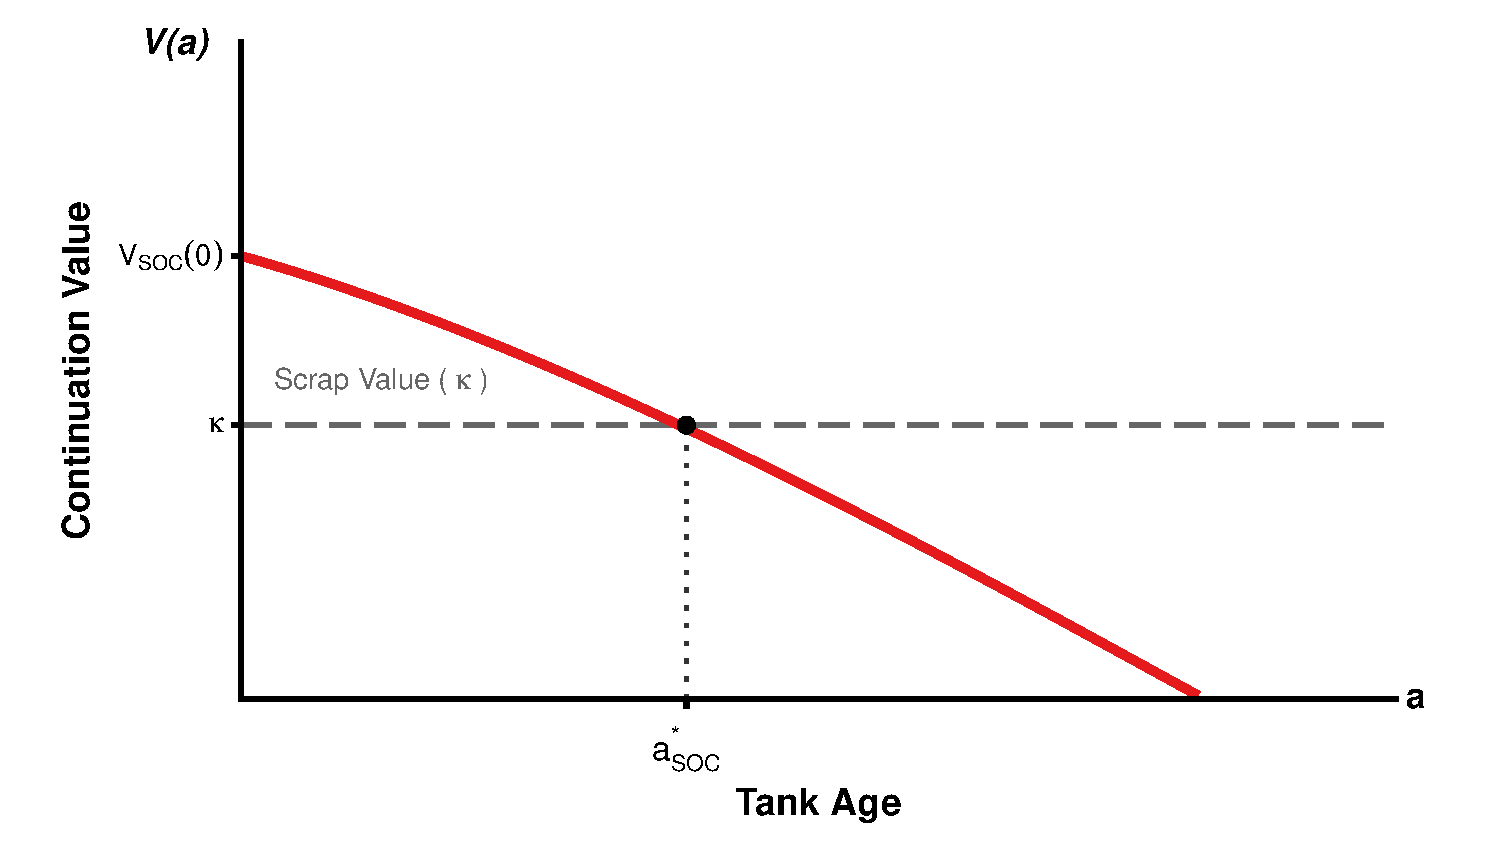
\includegraphics[height=0.78\textheight,keepaspectratio]{../../Output/Figures/Slide_Fig_2_SOC_Exit.pdf}
\end{center}
\end{frame}

\begin{frame}{Risk-Based vs.~Social Optimum}
\phantomsection\label{risk-based-vs.-social-optimum}
\BerkeleyLightMode

\vspace{0.2cm}
\begin{center}
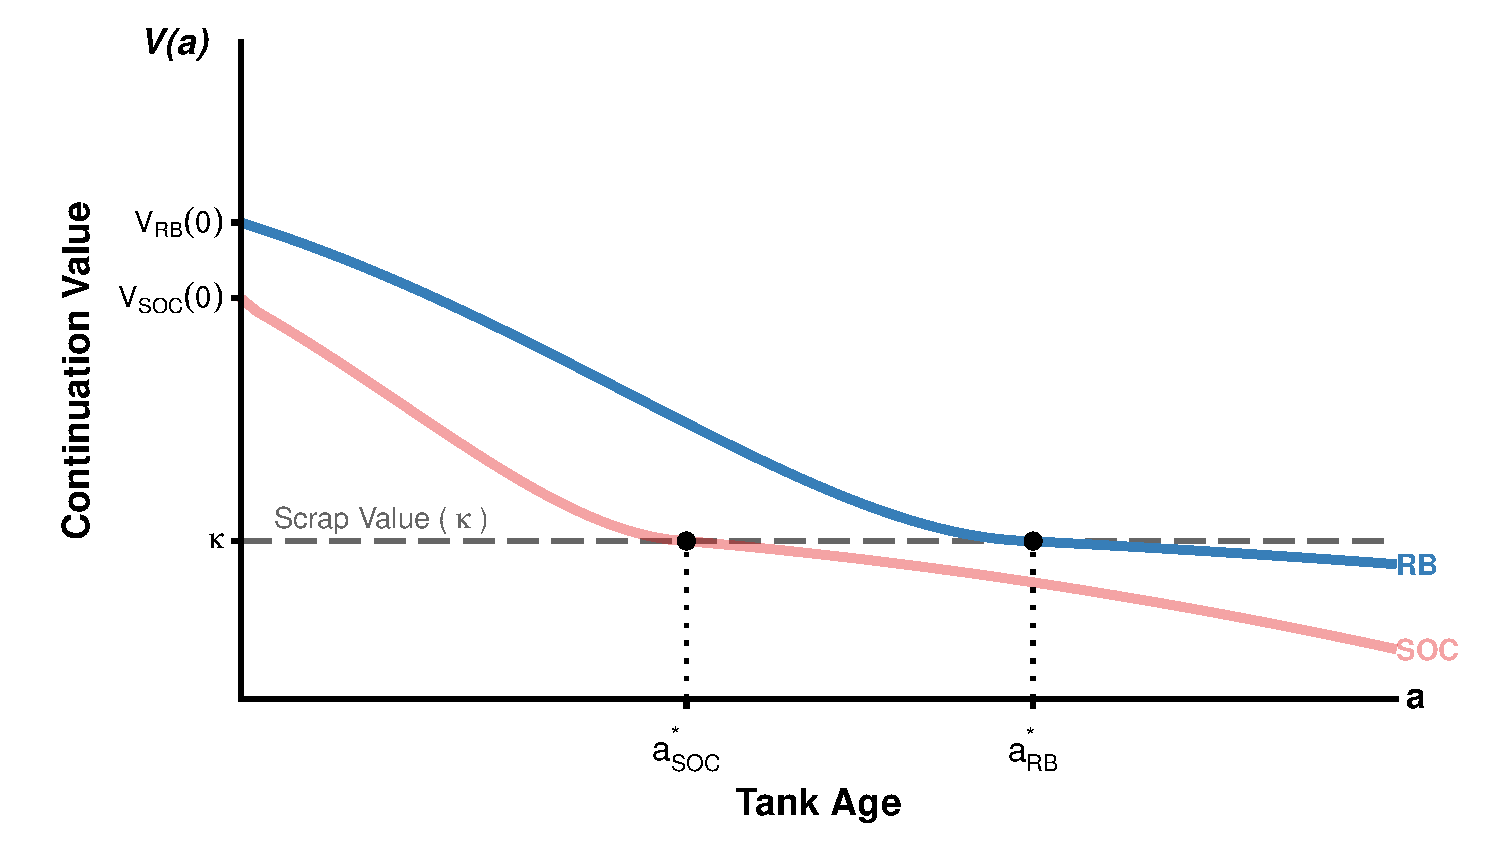
\includegraphics[height=0.78\textheight,keepaspectratio]{../../Output/Figures/Slide_Fig_3_SOC_RB_Comparison.pdf}
\end{center}
\end{frame}

\begin{frame}{Uniform Premium vs.~Social Optimum}
\phantomsection\label{uniform-premium-vs.-social-optimum}
\BerkeleyLightMode

\vspace{0.2cm}
\begin{center}
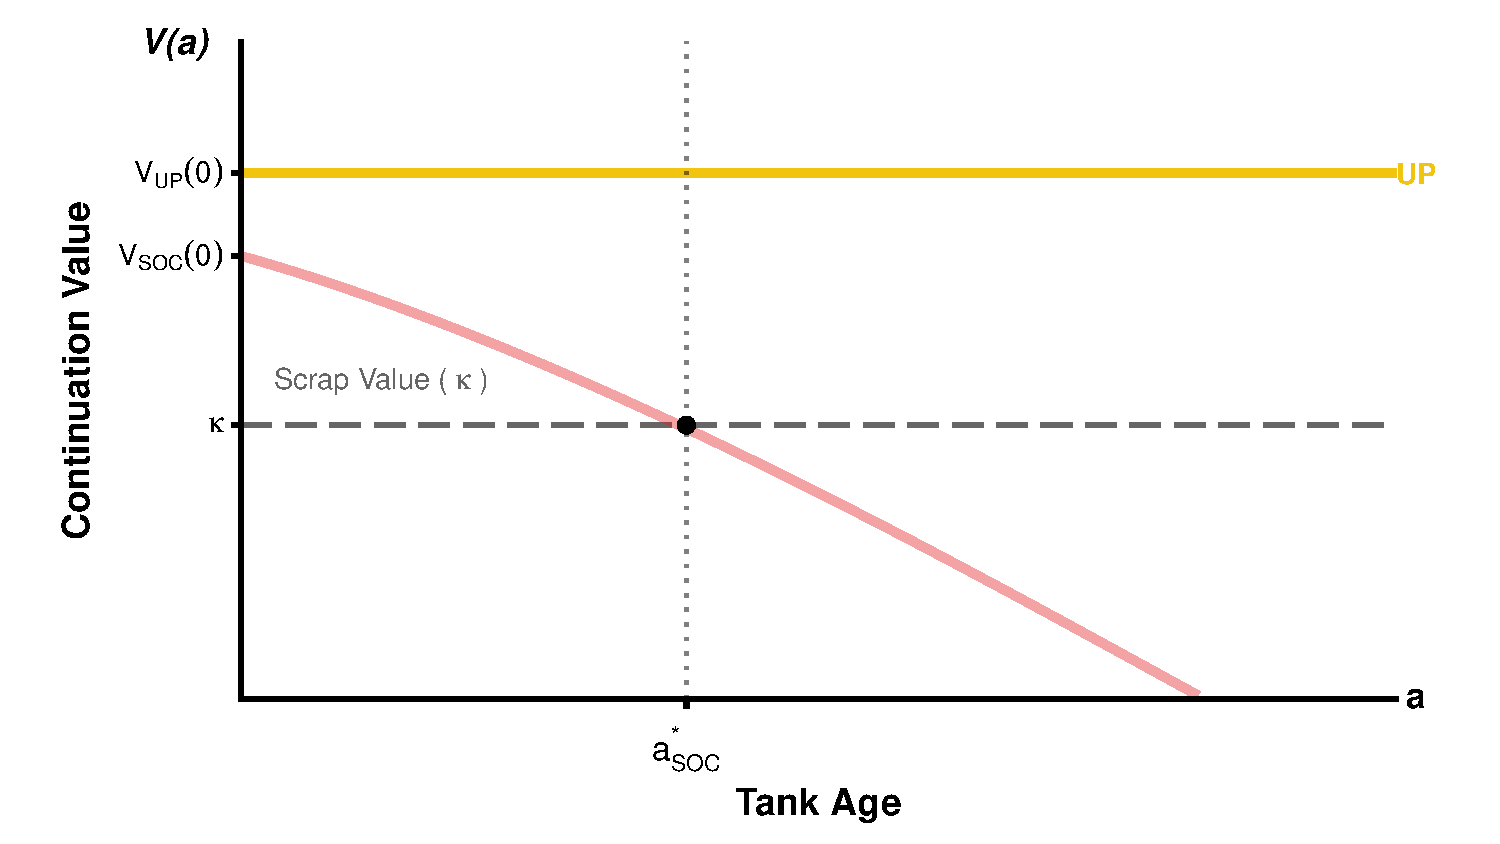
\includegraphics[height=0.78\textheight,keepaspectratio]{../../Output/Figures/Slide_Fig_5_SOC_FF_Comparison.pdf}
\end{center}
\end{frame}

\begin{frame}{Deadweight Loss Across Regimes}
\phantomsection\label{deadweight-loss-across-regimes}
\BerkeleyLightMode

\vspace{0.2cm}
\begin{center}
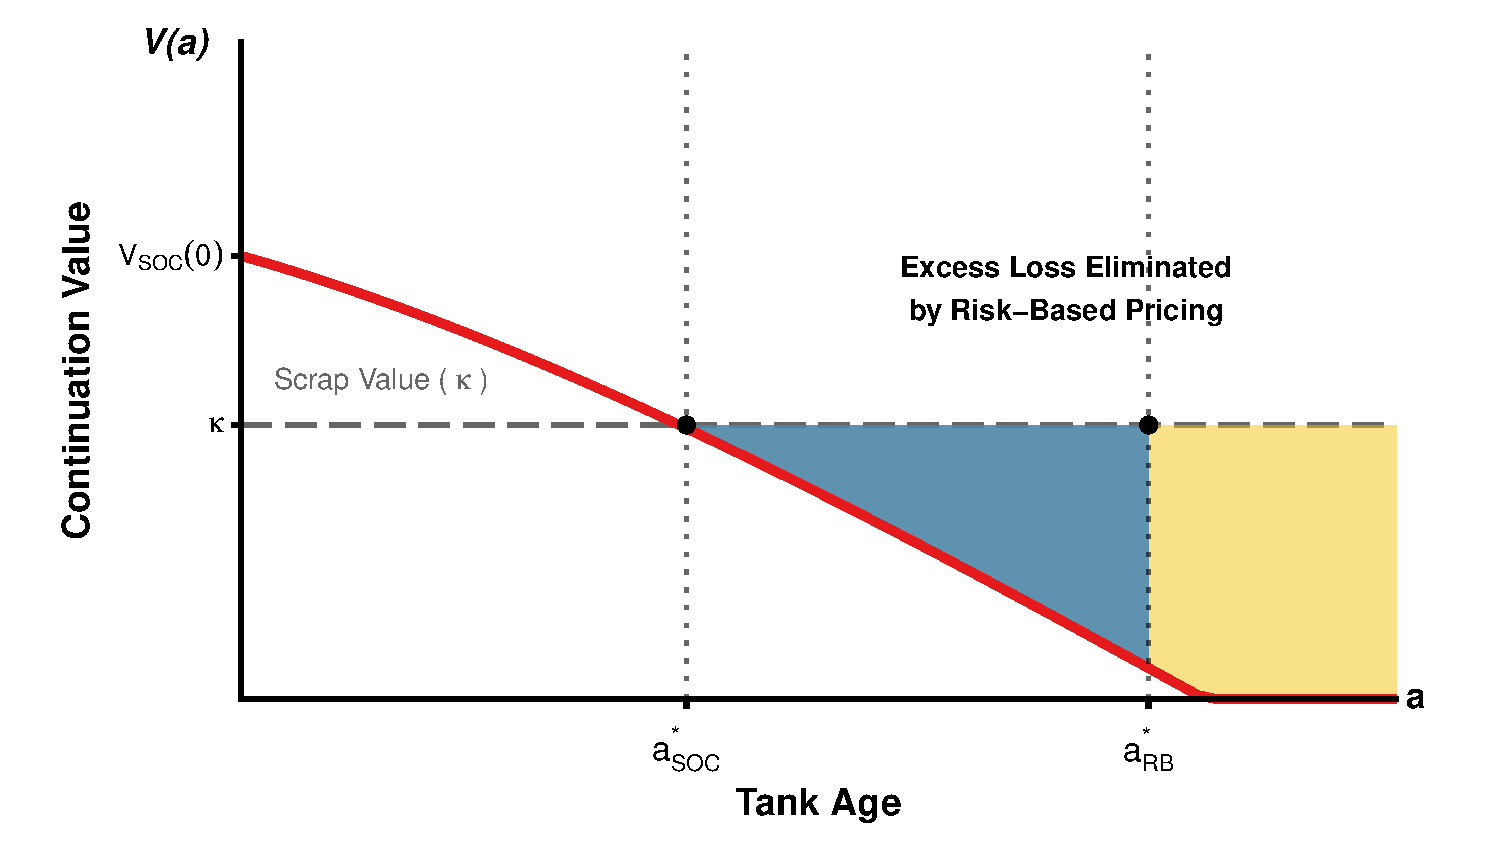
\includegraphics[height=0.78\textheight,keepaspectratio]{../../Output/Figures/Slide_Fig_7_Combined_DWL.pdf}
\end{center}
\end{frame}

\begin{frame}{}
\phantomsection\label{section-1}
\BerkeleyMode

\begin{center}
\Huge \textbf{Data \& Descriptive Evidence}
\end{center}
\end{frame}

\begin{frame}{FR Compliance: TX is a Private-Insurance Market}
\phantomsection\label{fr-compliance-tx-is-a-private-insurance-market}
\BerkeleyLightMode

\vspace{0.2cm}
\begin{center}
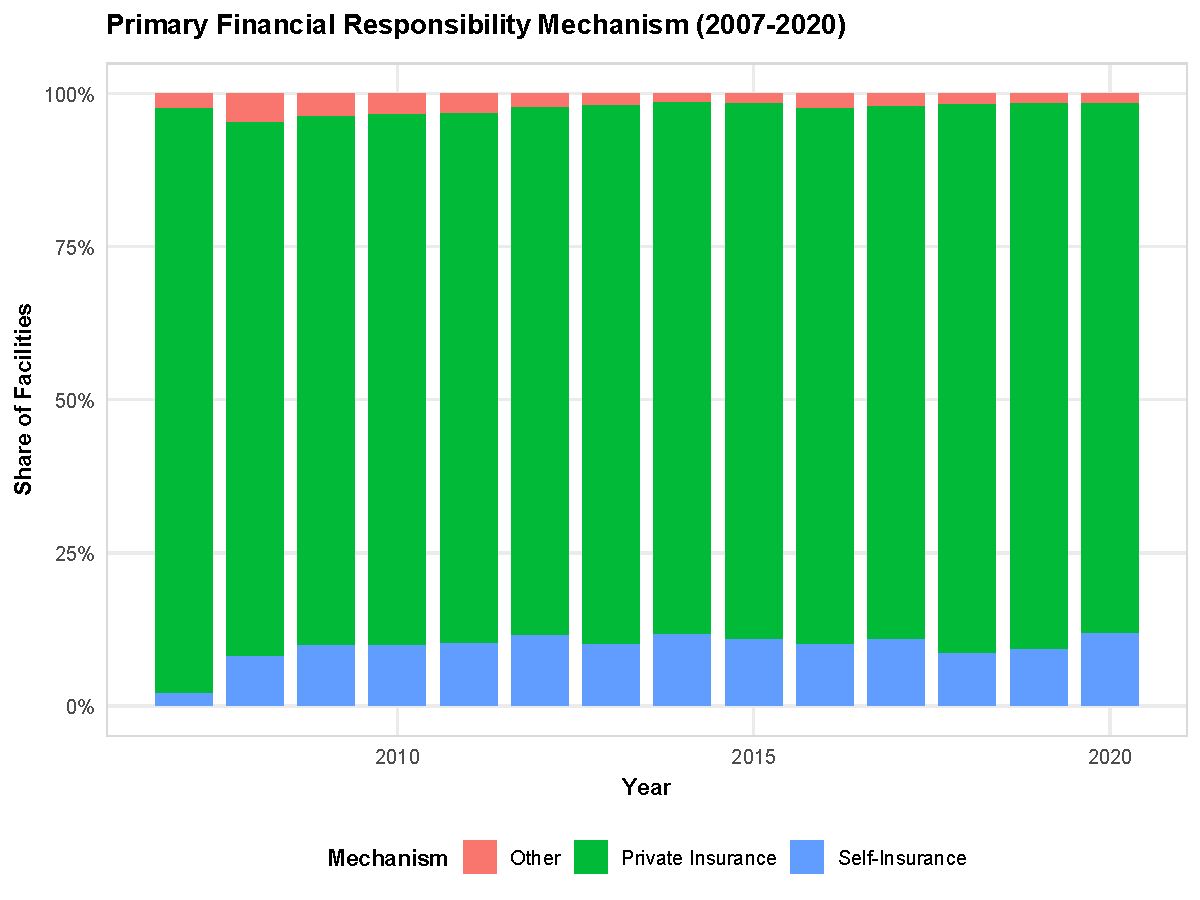
\includegraphics[height=0.78\textheight,keepaspectratio]{../../Output/Figures/FigureA_TX_FR_Coverage_Composition.pdf}
\end{center}
\end{frame}

\begin{frame}{Market Structure: Concentrated and Stable}
\phantomsection\label{market-structure-concentrated-and-stable}
\BerkeleyLightMode

\vspace{0.2cm}
\begin{center}
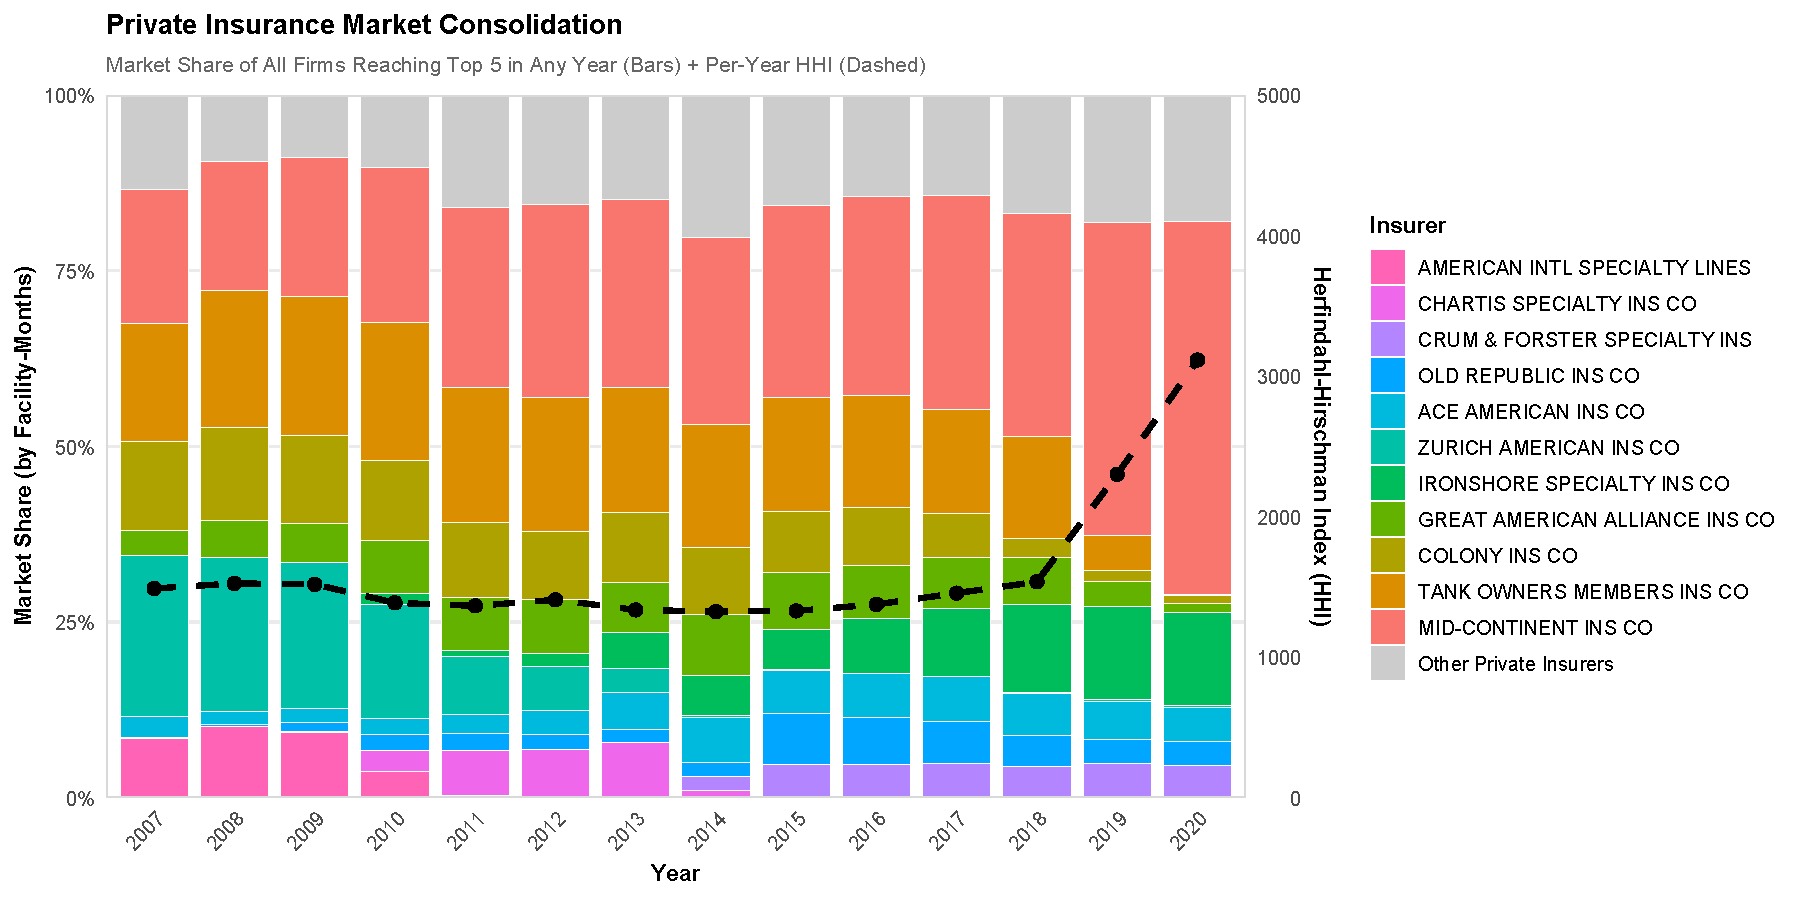
\includegraphics[height=0.78\textheight,keepaspectratio]{../../Output/Figures/Figure_TX_FR_Top5_Dominance_HHI.pdf}
\end{center}
\end{frame}

\begin{frame}{Premium Construction}
\phantomsection\label{premium-construction}
\BerkeleyLightMode

\textbf{Texas} --- rebuilt from Mid-Continent Casualty rate filings
(SERFF, 2006--2024):

\[P_{ijt} \;=\; \text{Base}_t \;\times\; \text{ILF}_{it} \;\times\; \Bigl(1 \;+\; \sum_{k} \lambda_{k,t}\, X_{ijt,k}\Bigr)\]

\begin{itemize}
\tightlist
\item
  \(\text{Base}_t\): per-tank base rate, four filing periods
\item
  \(\text{ILF}_{it}\): increased-limit factor; fix coverage at
  federal-minimum \$1M/\$1M
\item
  \(X_{ijt}\): tank age, wall, piping, leak-detection technology
\item
  \(\lambda_{k,t}\): additive credits/debits from the filed schedule
\end{itemize}

\textbf{Control states} --- state financial-responsibility fund records:
a per-tank annual assessment, largely flat across years and tank
characteristics.
\end{frame}

\begin{frame}{Premium Levels: Texas vs.~Control States}
\phantomsection\label{premium-levels-texas-vs.-control-states}
\BerkeleyLightMode

\vspace{0.2cm}
\begin{center}
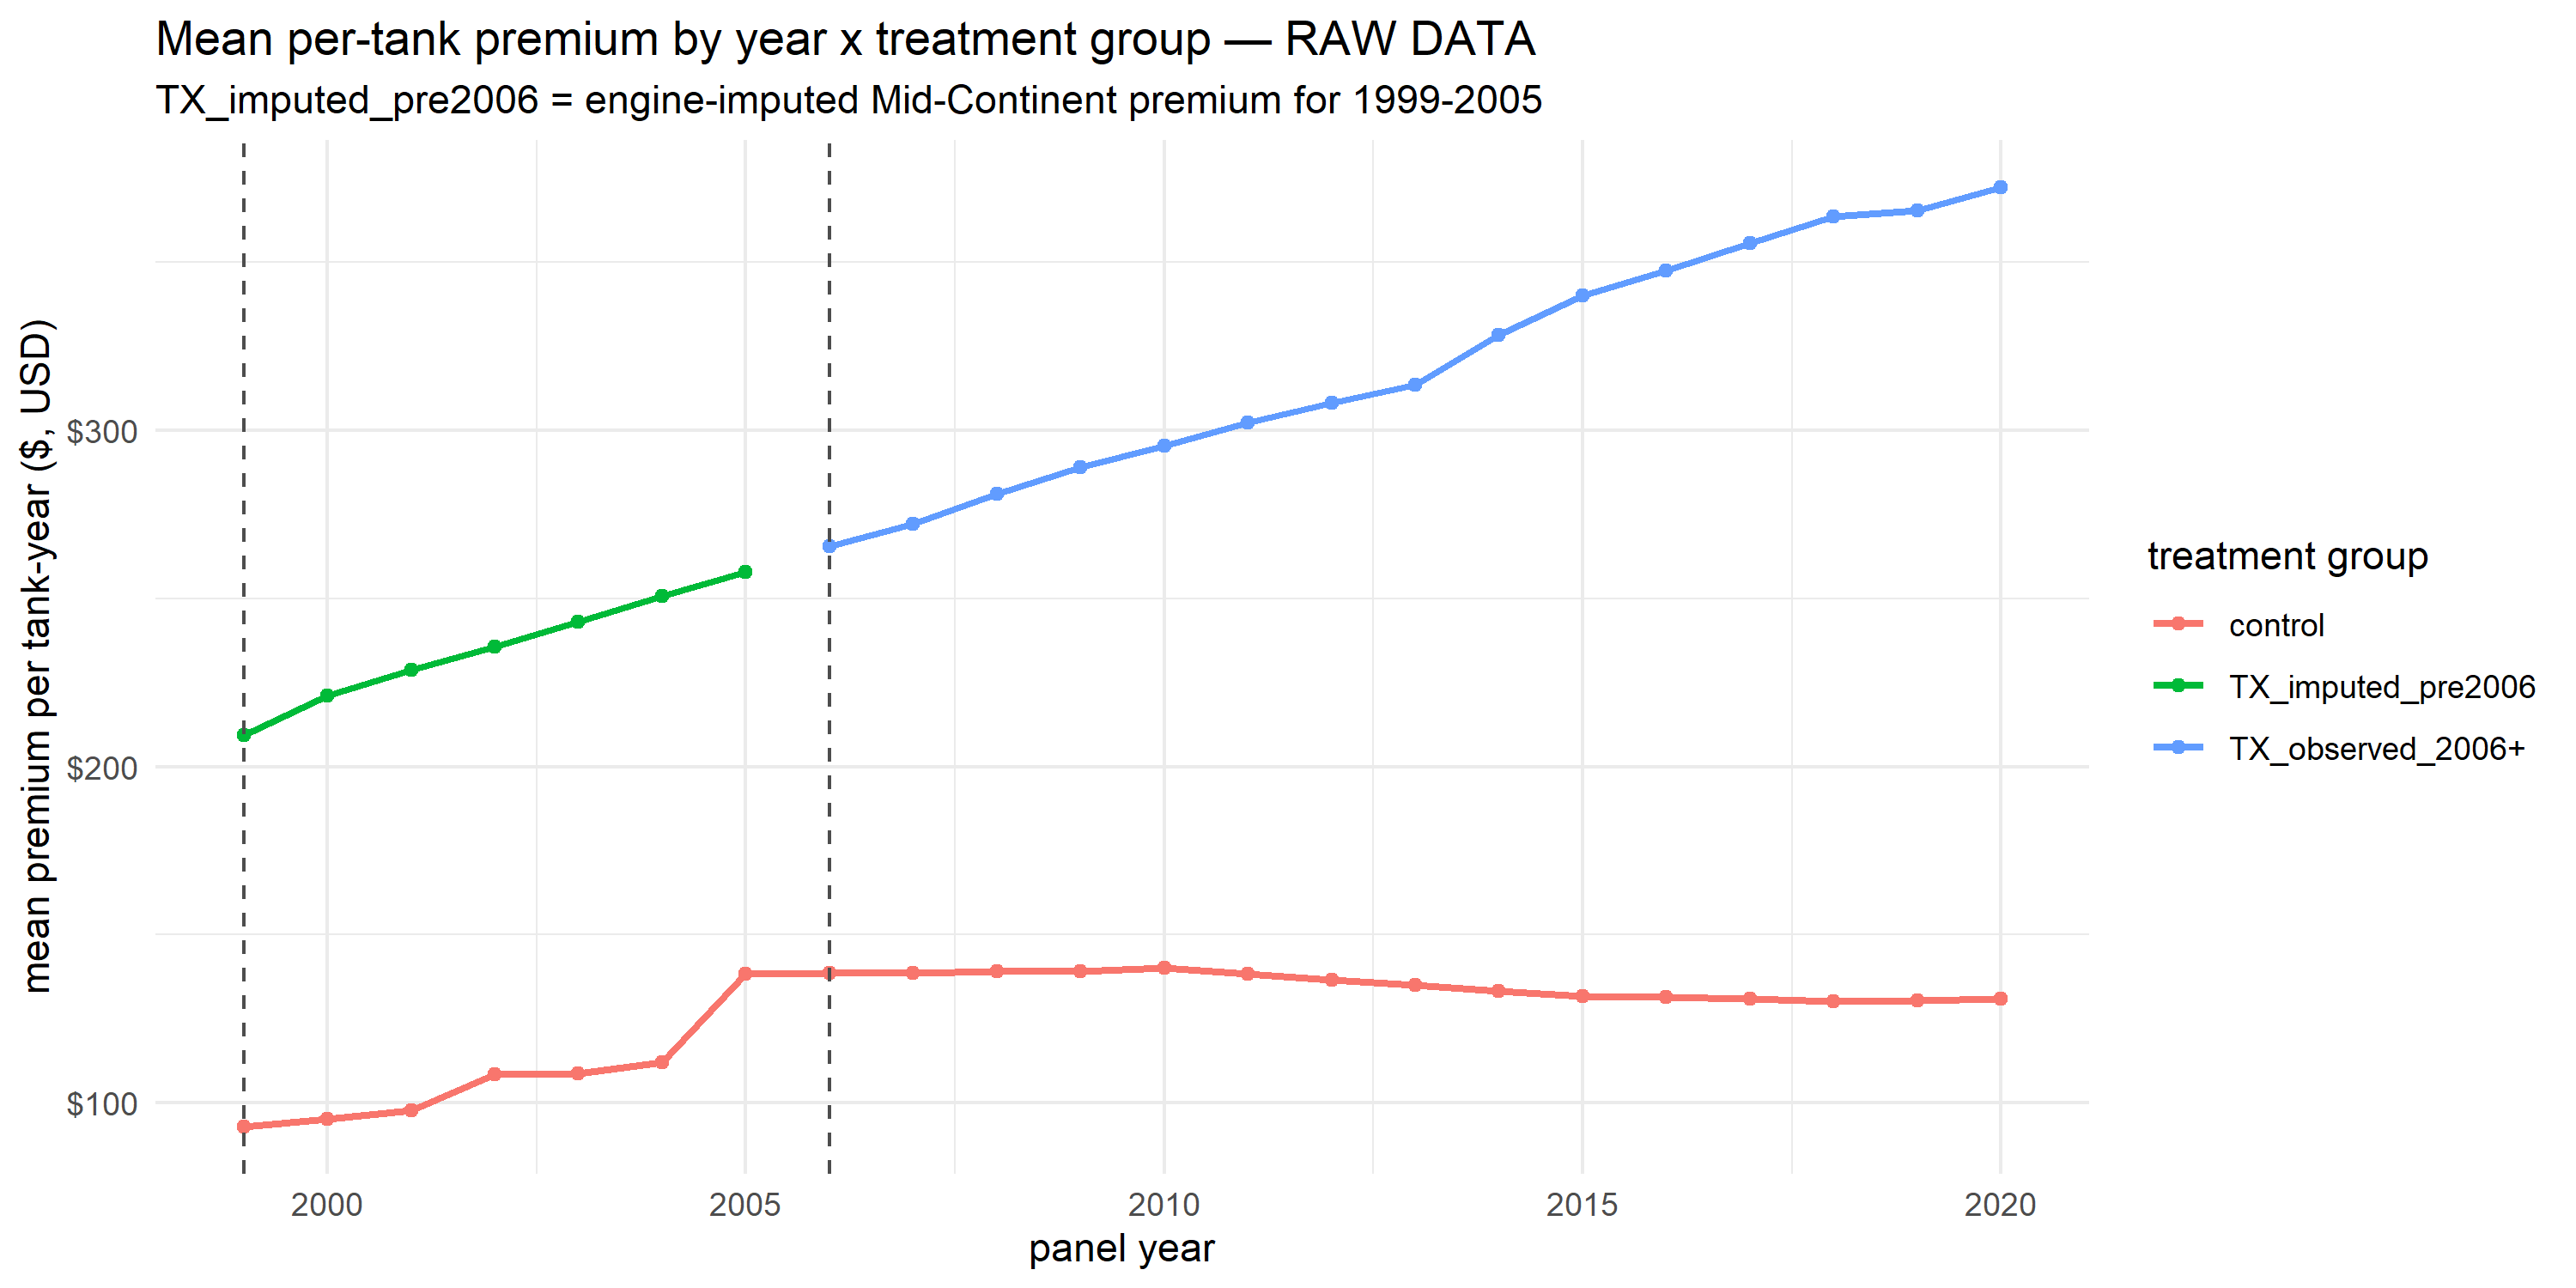
\includegraphics[height=0.78\textheight,keepaspectratio]{../../Output/Figures/04e_Premium_by_Year_Treatment.png}
\end{center}
\end{frame}

\begin{frame}{Risk Prediction: Setup}
\phantomsection\label{risk-prediction-setup}
\BerkeleyLightMode

\textbf{Estimand.} Annual first-release hazard in the never-yet-leaked
risk set:

\[h(t \mid x) \;=\; P\bigl(\,\text{first confirmed release in year } t \mid \text{no prior release}, \; x\,\bigr)\]

In plain words: given what an underwriter can observe at the start of a
policy year, what's the probability of a claim?

\textbf{Model.} Penalized logistic regression on the pre-treatment
panel:

\begin{itemize}
\tightlist
\item
  \(x\): 3-year age bins fully interacted with wall construction; state
  FE; fuel and portfolio controls
\item
  Lasso variable selection; inverse-frequency weights for the 0.70\%
  base rate
\item
  Out-of-sample CV (10 folds); post-hoc recalibration to the empirical
  event rate
\end{itemize}

\textbf{Sample.} 3.93M pre-treatment facility-years; \(27{,}455\)
confirmed first-release events.

\(\hat h(x)\) feeds the next figure and the structural-model hazard
\(h(a_t, W_i)\).
\end{frame}

\begin{frame}{Single-Walled Tanks Drive the Age--Hazard Gradient}
\phantomsection\label{single-walled-tanks-drive-the-agehazard-gradient}
\BerkeleyLightMode

\vspace{0.2cm}
\begin{center}
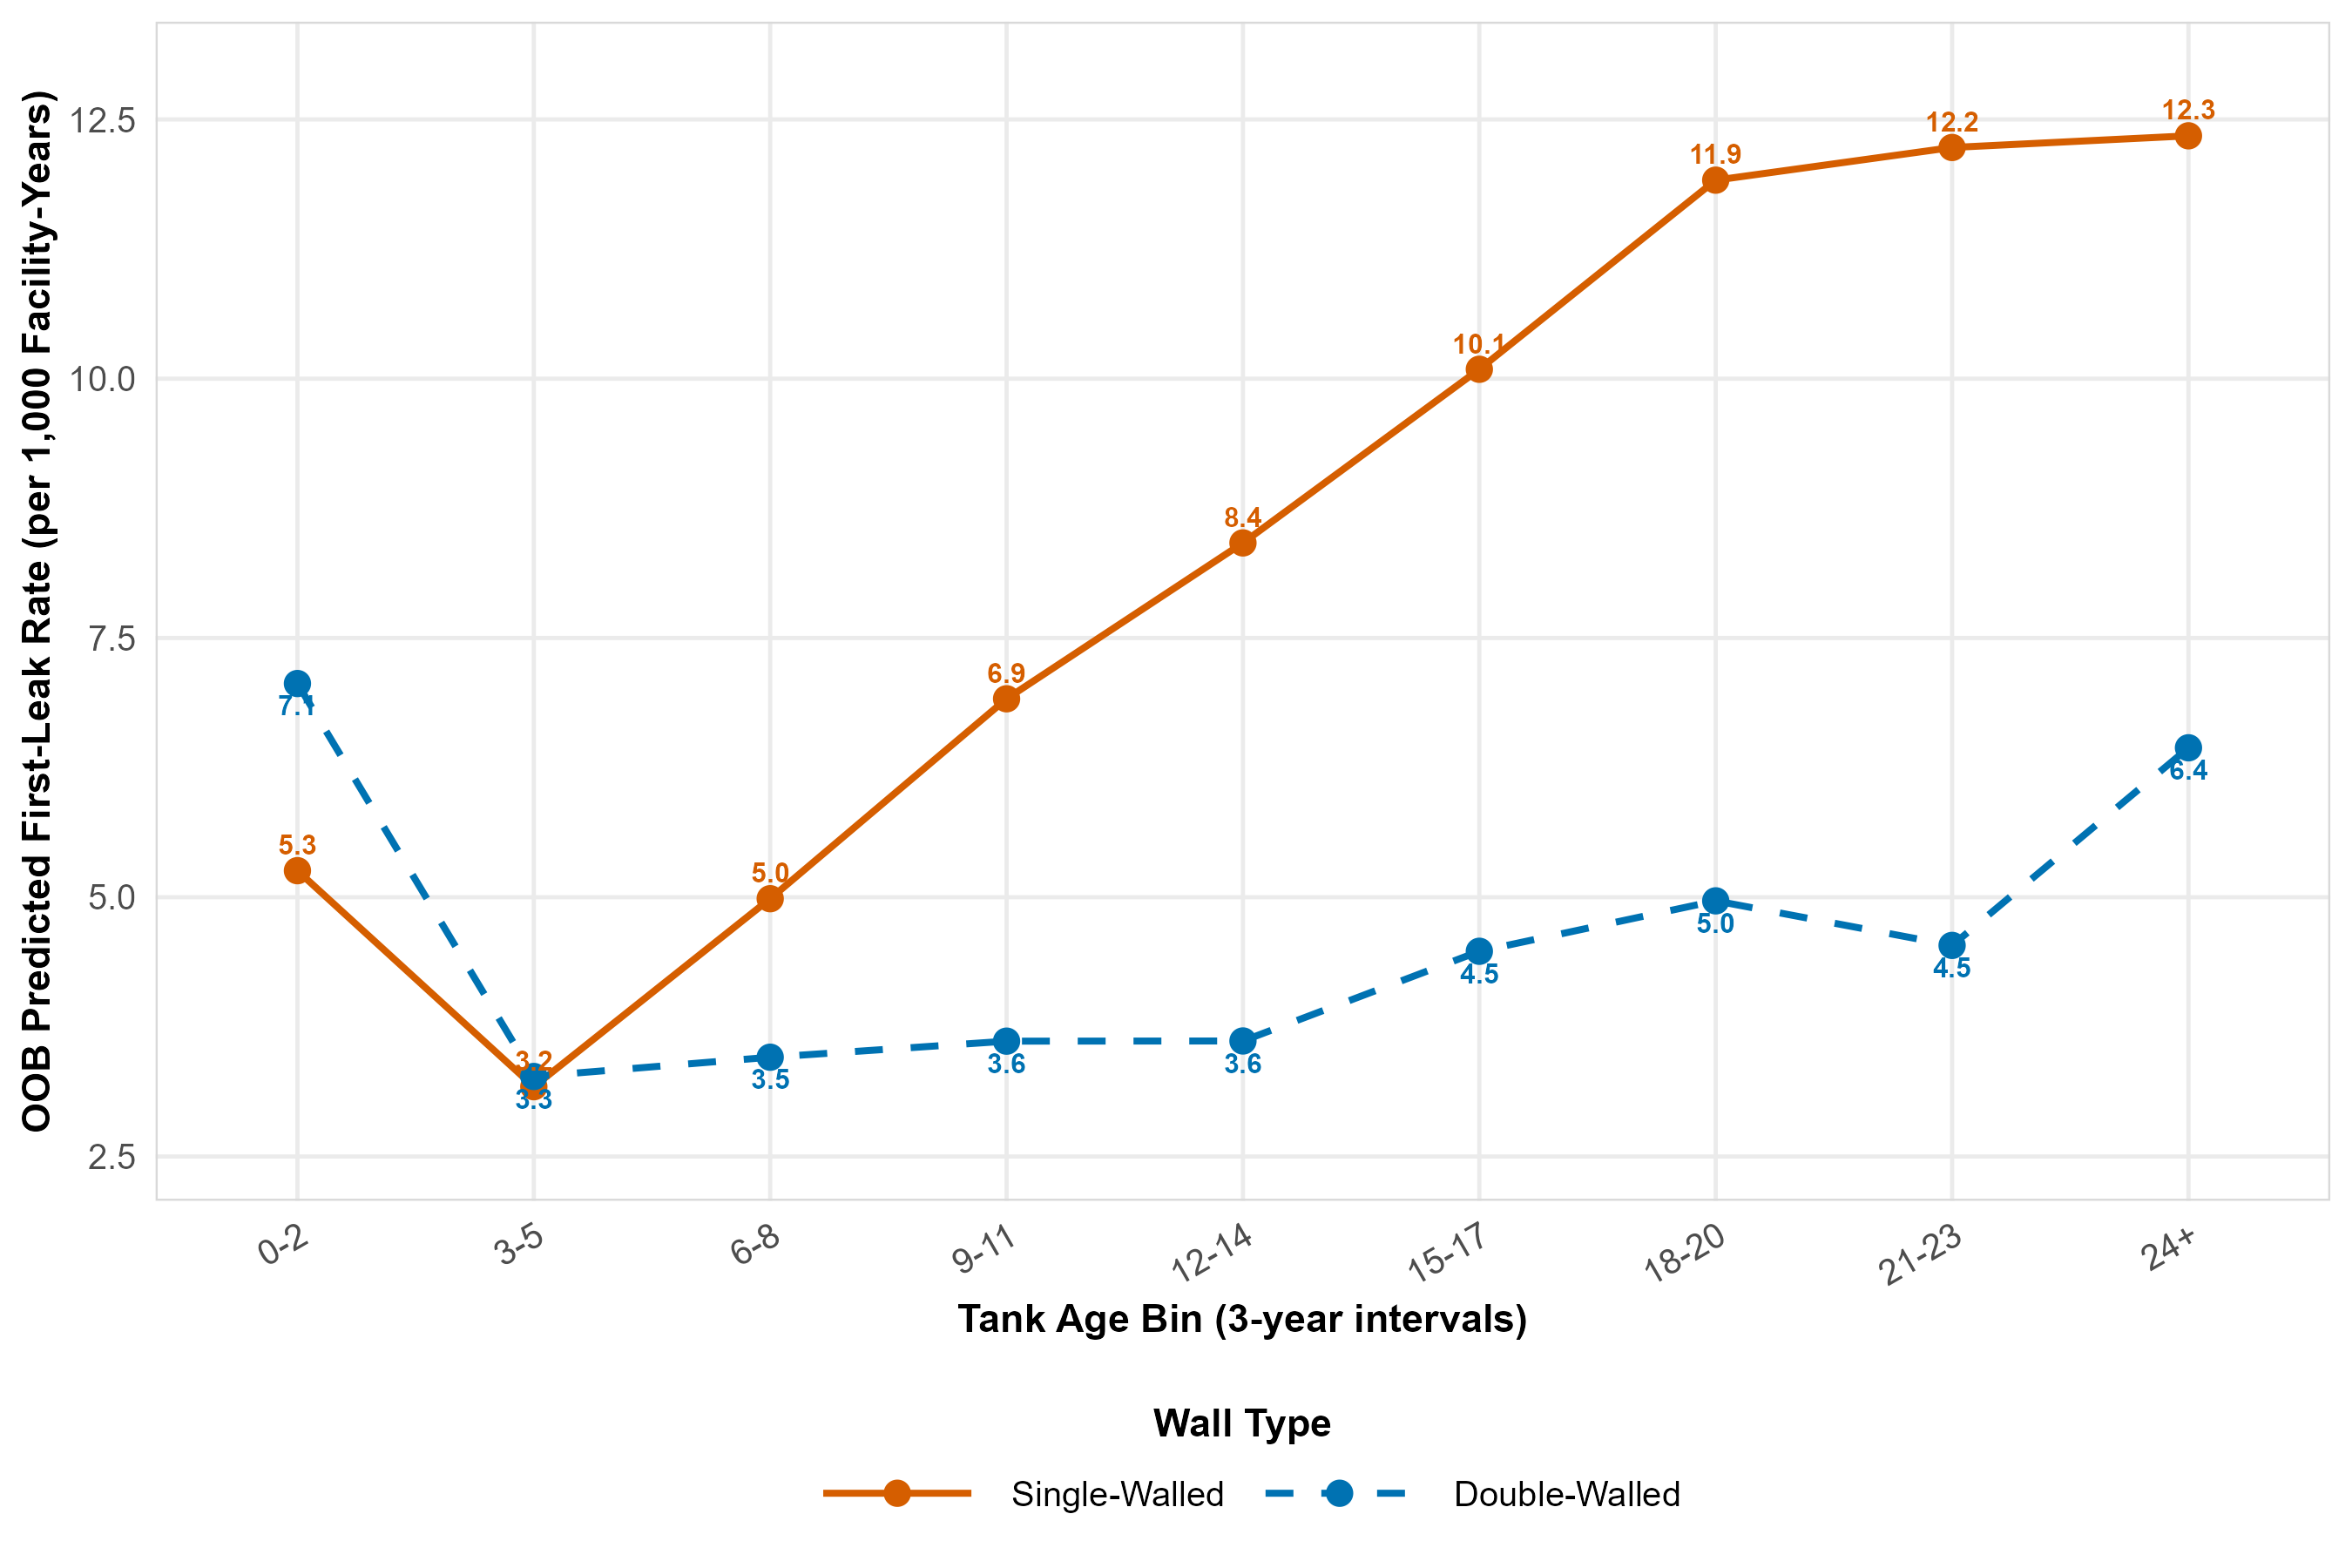
\includegraphics[height=0.78\textheight,keepaspectratio]{../../Output/Figures/Figure_CV_CellRisk.png}
\end{center}

\begin{tikzpicture}[remember picture, overlay]
\node[anchor=south west, inner sep=0pt] at ([xshift=10pt, yshift=10pt]current page.south west) {%
  \navbutton[cell-gof][fill=BerkeleyBlue, font=\tiny, inner sep=2pt]{Goodness of fit $\rightarrow$}%
};
\end{tikzpicture}
\end{frame}

\begin{frame}{Premiums Track the Risk We Can Predict}
\phantomsection\label{premiums-track-the-risk-we-can-predict}
\BerkeleyLightMode

\vspace{0.1cm}
\begin{center}
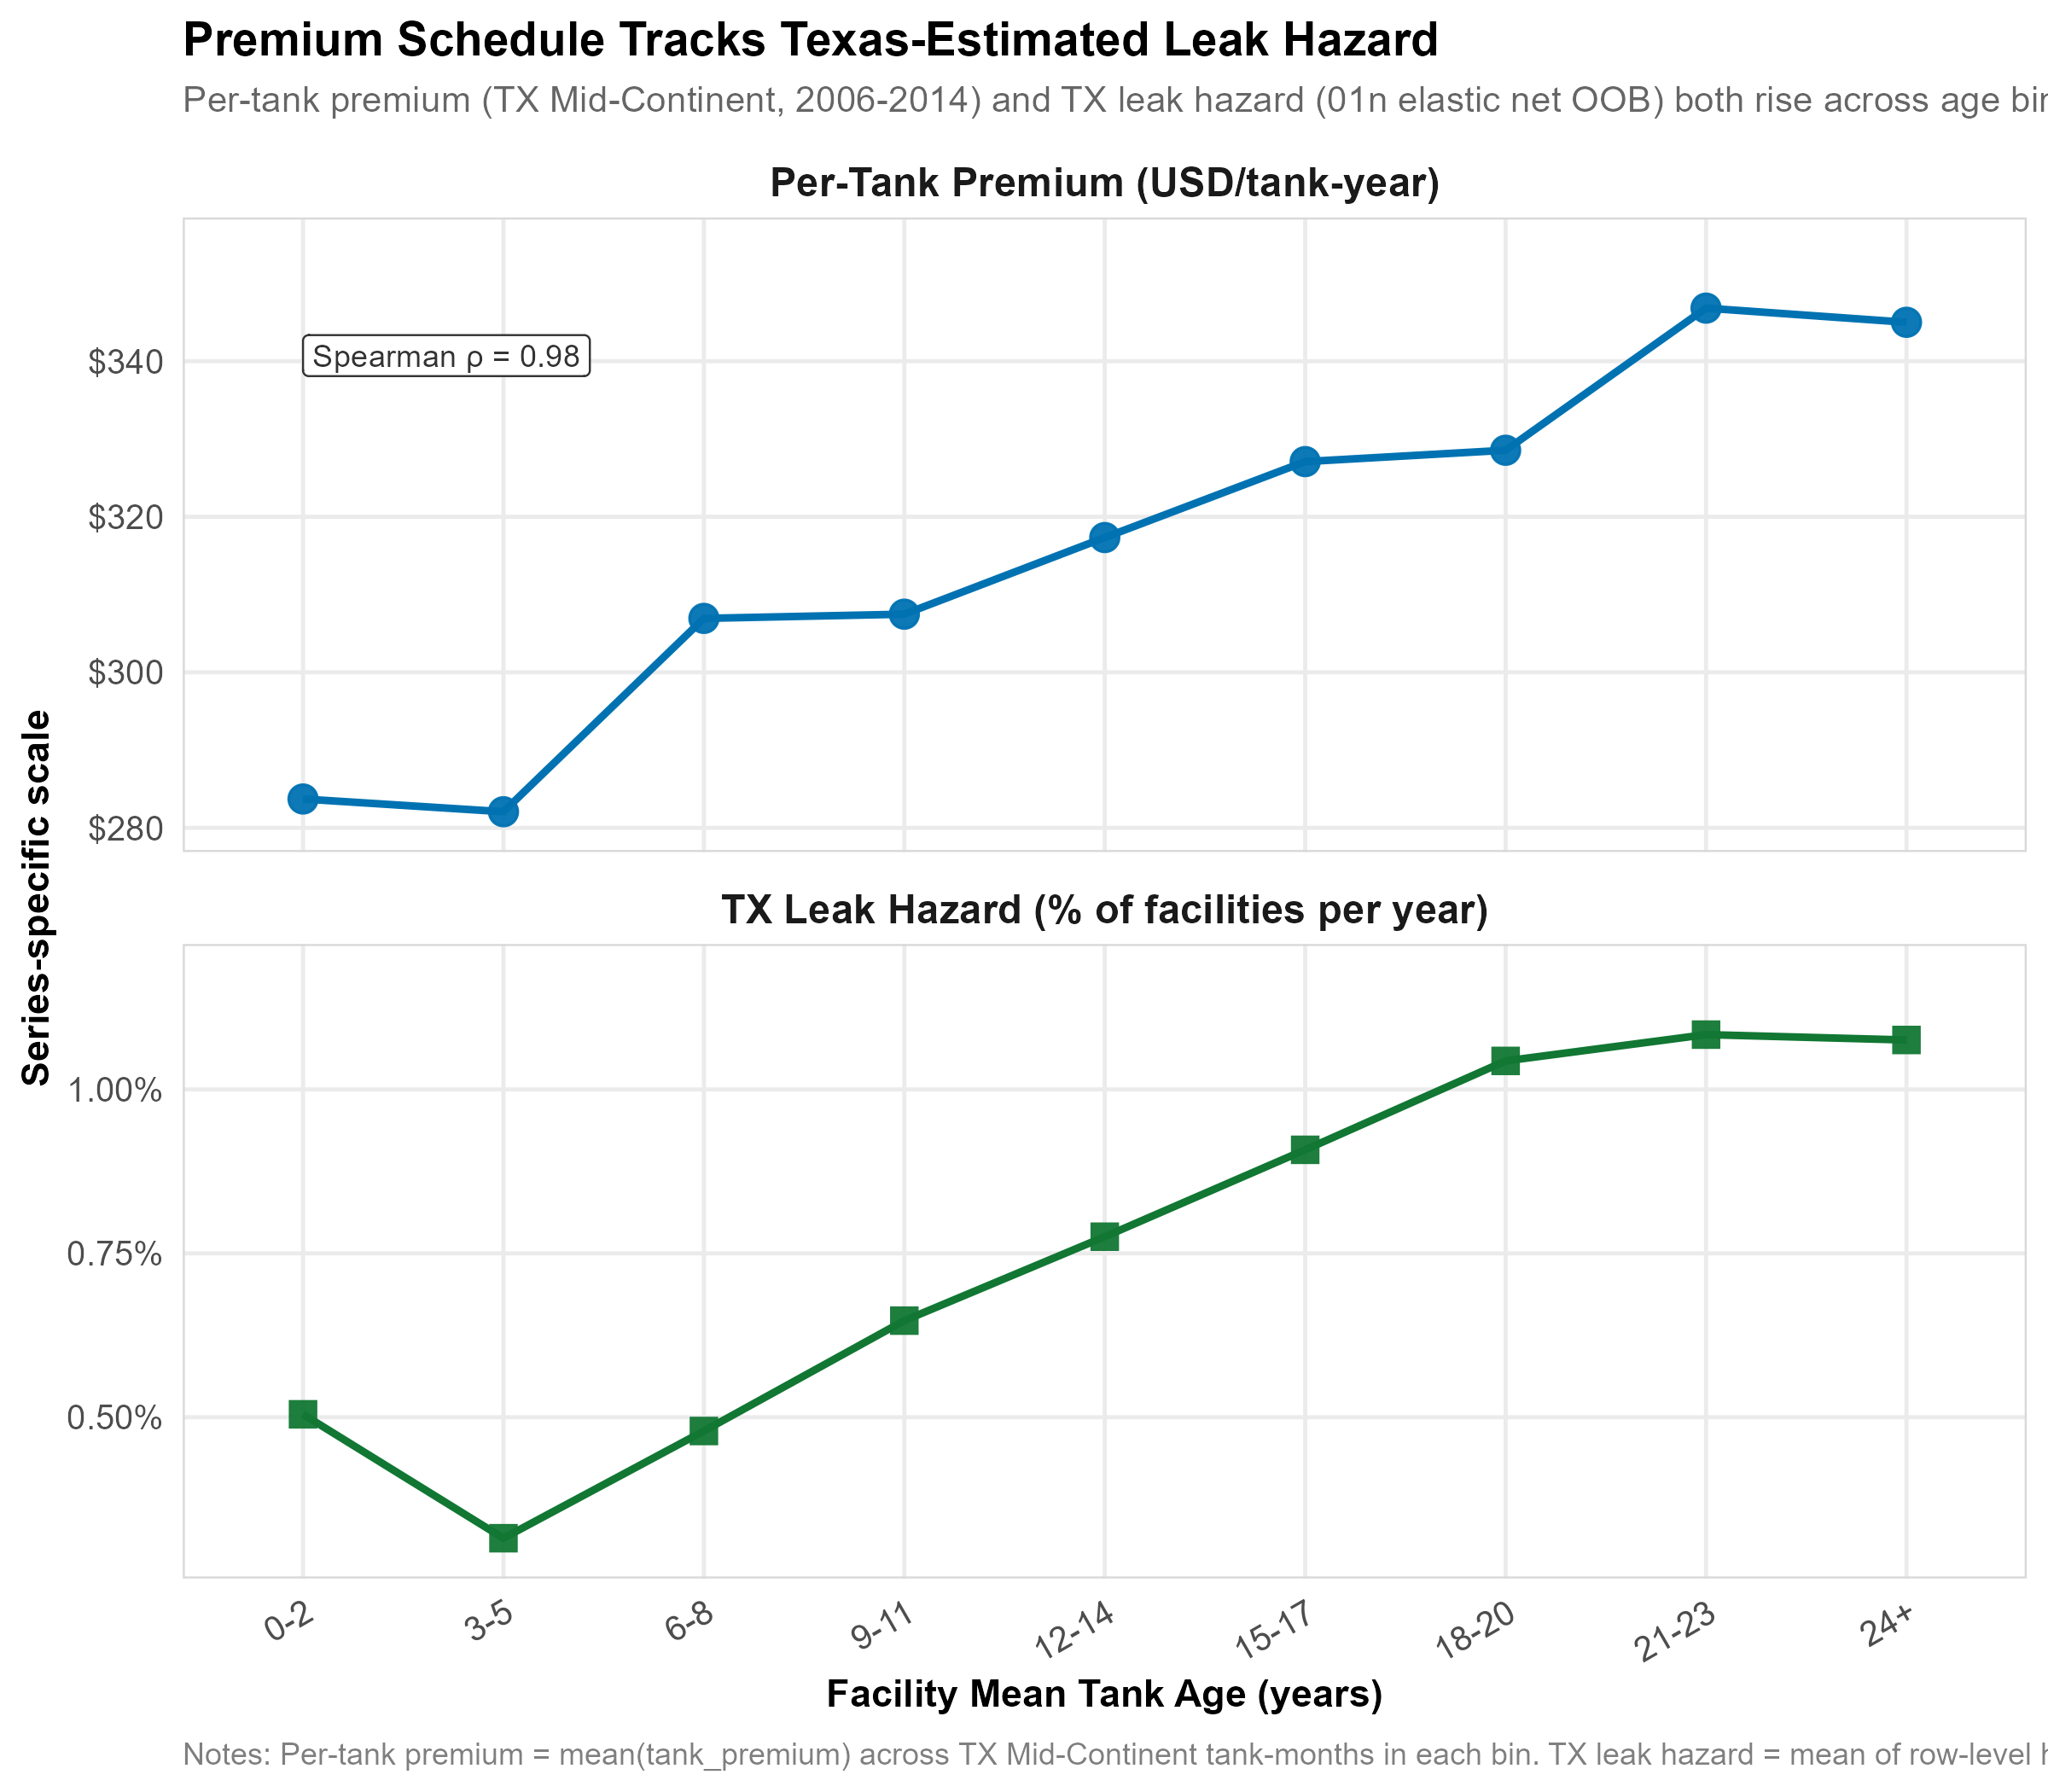
\includegraphics[height=0.80\textheight,keepaspectratio]{../../Output/Figures/Figure_Premium_vs_Hazard_Raw.png}
\end{center}

\begin{tikzpicture}[remember picture, overlay]
\node[anchor=south west, inner sep=0pt] at ([xshift=10pt, yshift=10pt]current page.south west) {%
  \navbutton[premium-vs-el][fill=BerkeleyBlue, font=\tiny, inner sep=2pt]{Predicted per-tank EL $\rightarrow$}%
};
\end{tikzpicture}
\end{frame}

\begin{frame}{Cleanup Cost Distribution}
\phantomsection\label{cleanup-cost-distribution}
\BerkeleyLightMode

\vspace{0.2cm}
\begin{center}
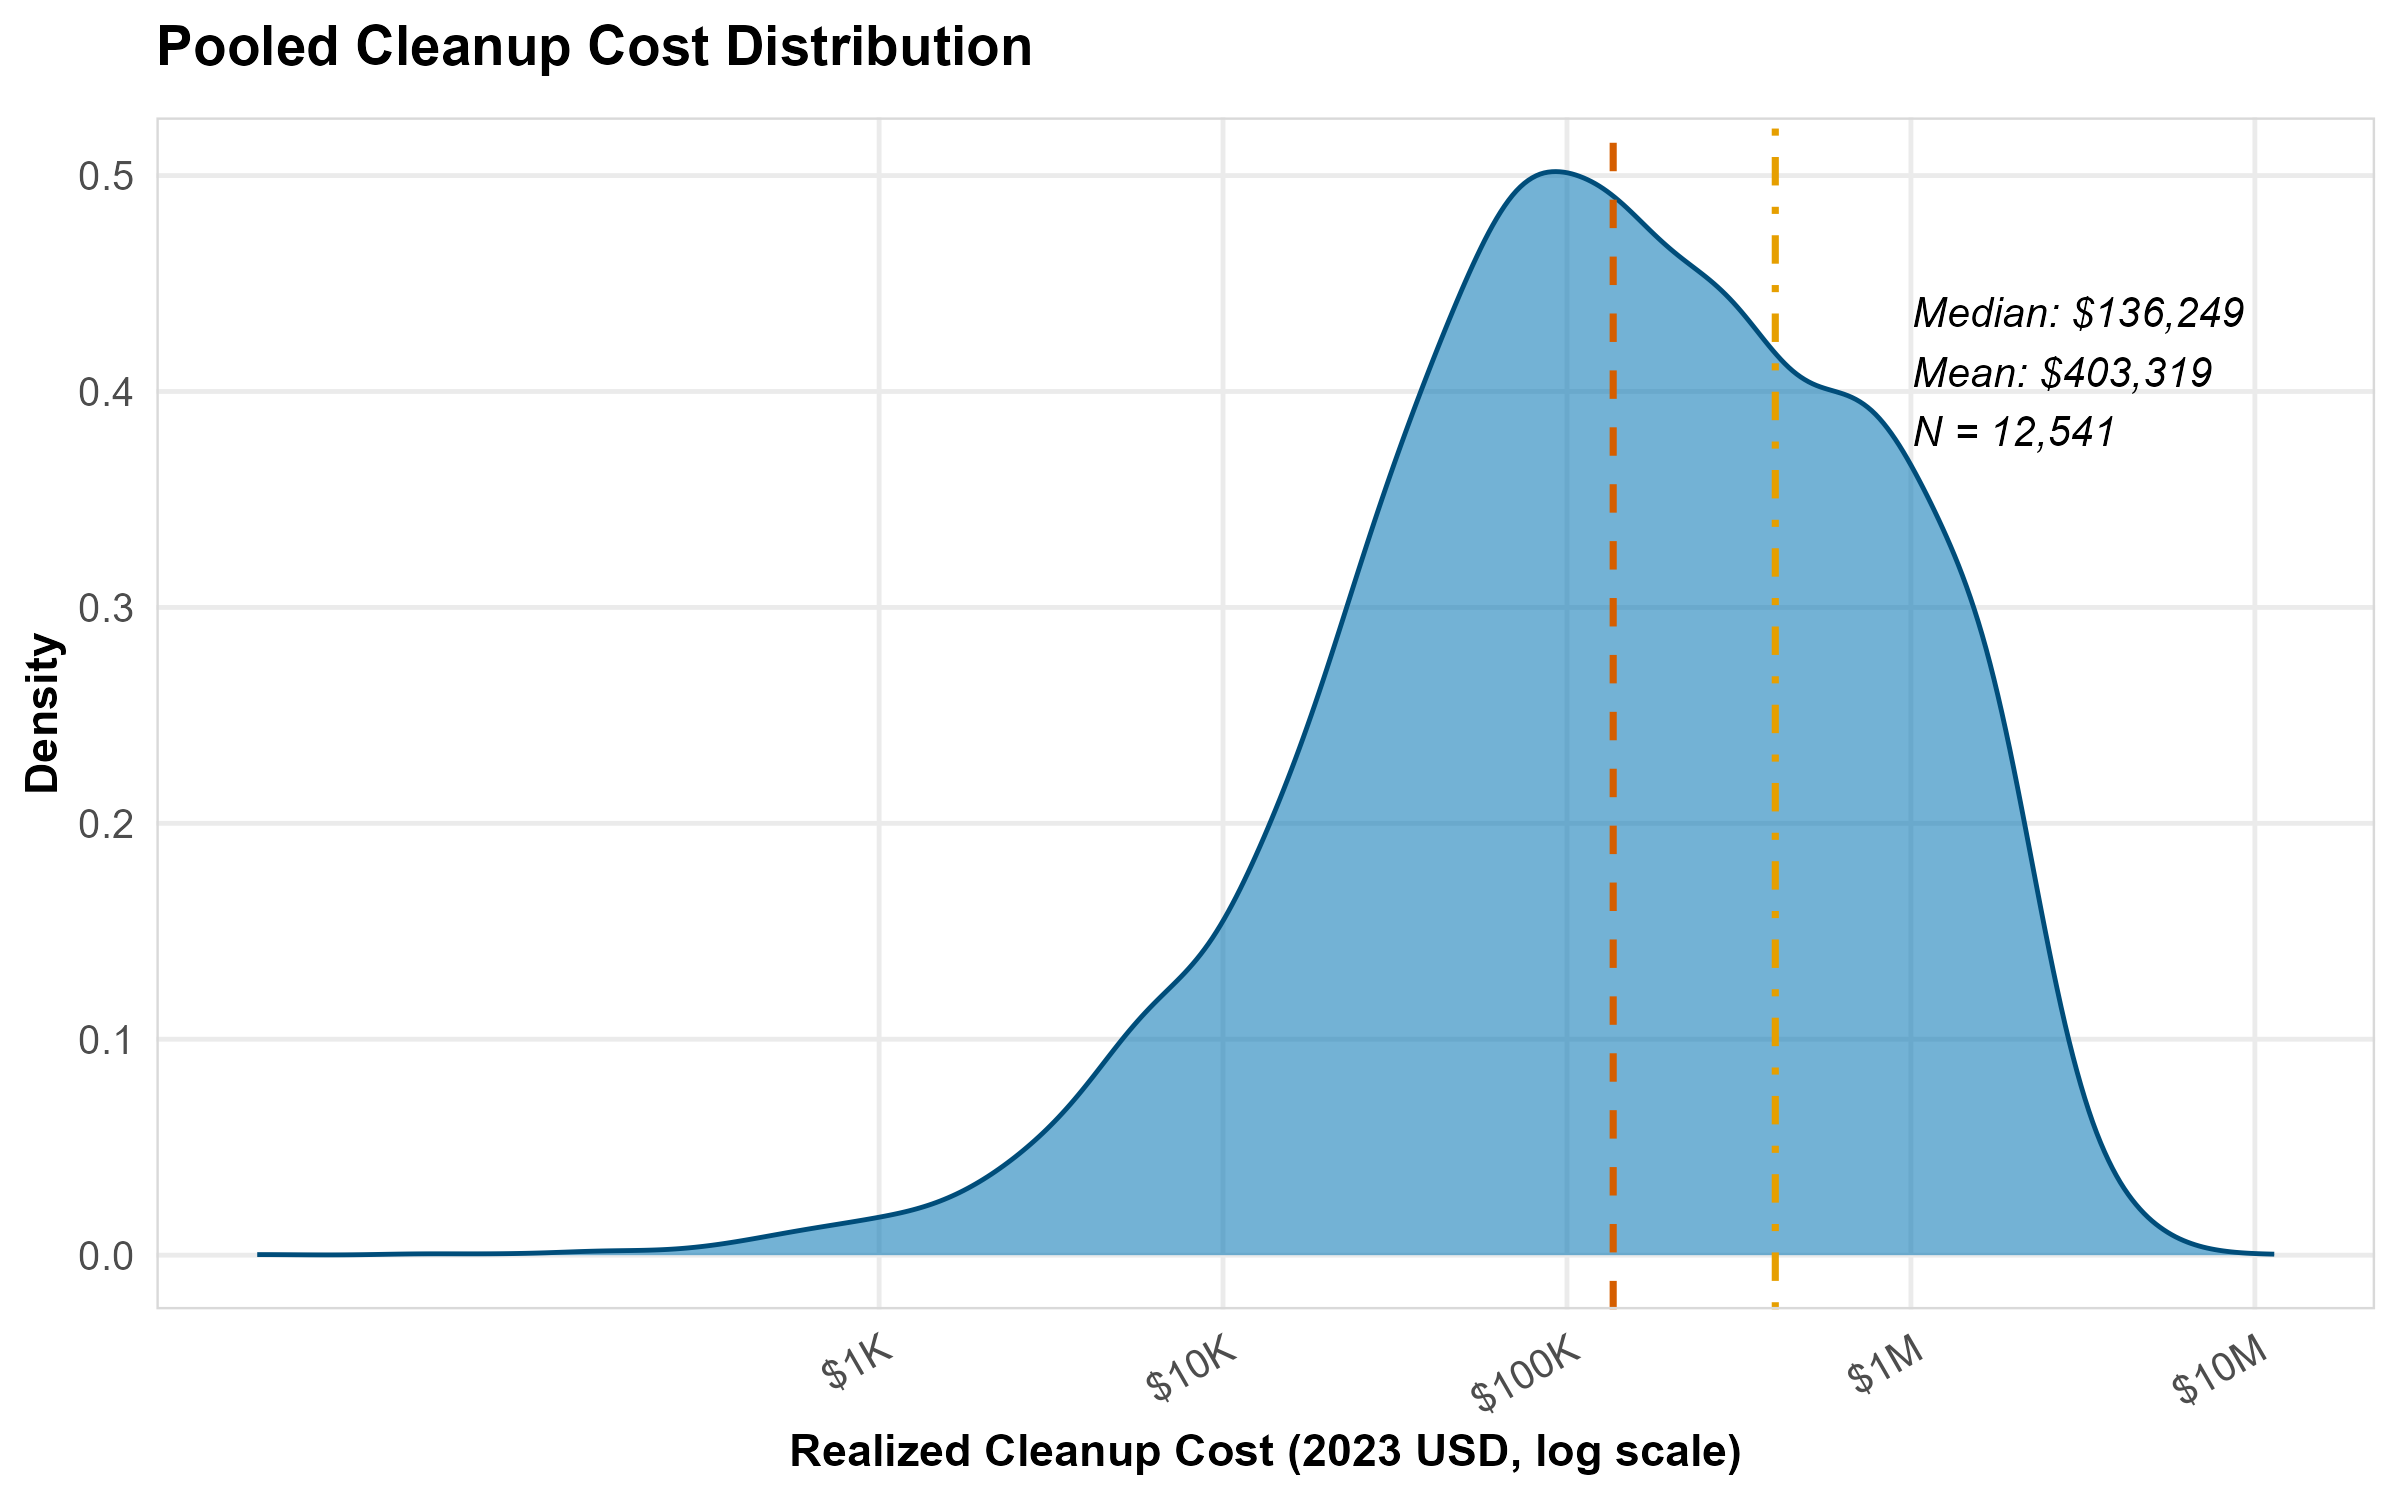
\includegraphics[height=0.78\textheight,keepaspectratio]{../../Output/Figures/Figure_cost_distribution_pooled.png}
\end{center}
\end{frame}

\begin{frame}{}
\phantomsection\label{section-2}
\BerkeleyMode

\begin{center}
\Huge \textbf{Reduced Form Evidence}
\end{center}
\end{frame}

\begin{frame}{Sample Descriptive Statistics}
\phantomsection\label{sample-descriptive-statistics}
\BerkeleyLightMode

\vspace{0.15cm}
\begin{center}
\scriptsize
\small
\renewcommand{\arraystretch}{1.1}
\begin{tabular}{lcc}
\toprule
 & Texas & 17 control states \\
\midrule
\multicolumn{3}{l}{\textit{Panel size}} \\
Facility-years (incumbent, 1985--2018) & 870{,}341 & 3{,}782{,}424 \\
Tank-years (active-at-treatment)       & \multicolumn{2}{c}{9{,}761{,}982} \\
\midrule
\multicolumn{3}{l}{\textit{Tank stock at Dec 22, 1998 (per facility)}} \\
Facilities                             & 25,985 & 114,304 \\
Mean tanks                             & 2.78 & 2.74 \\
Single-walled share (tank-weighted)    & 89.1\% & 89.5\% \\
Mean oldest tank age, years            & 15.32 & 18.09 \\
Mean total capacity, gal               & 22,585 & 62,405 \\
Gasoline facility share                & 66.1\% & 75.4\% \\
\midrule
\multicolumn{3}{l}{\textit{Vintage composition (facility counts, full panel)}} \\
Pre-1989 vintage (faced EPA phase-in)   & \multicolumn{2}{c}{96{,}923} \\
Post-1988 vintage                       & \multicolumn{2}{c}{42{,}523} \\
\midrule
\multicolumn{3}{l}{\textit{Pre-reform annual rates (control mean)}} \\
Tank closure                            & --- & 2.03\%  \\
Leak discovery                          & --- & 1.73\%  \\
\midrule
\multicolumn{3}{p{0.86\linewidth}}{\textit{Control states:} AR, CO, ID, KS, KY, LA, MA, MD, ME, MN, MO, NC, OH, OK, SD, TN, VA.} \\
\multicolumn{3}{p{0.86\linewidth}}{\textit{Treatment:} Dec 22, 1998 (TX SB 1317 mandates third-party UST insurance). SEs clustered by state.} \\
\bottomrule
\end{tabular}

\end{center}
\end{frame}

\begin{frame}{Estimating Sample and Specification}
\phantomsection\label{estimating-sample-and-specification}
\BerkeleyLightMode

\textbf{Static DiD.}

\[Y_{it} \;=\; \beta\,(\text{Texas}_{f(i)} \times \text{Post}_t) \;+\; \alpha_i \;+\; \delta_{ct} \;+\; \varepsilon_{it}\]

\textbf{Event study.}

\[Y_{it} \;=\; \sum_{\tau \neq -1} \beta_\tau \cdot \bigl(\text{Texas}_{f(i)} \times \mathbf{1}[t - 1998 = \tau]\bigr) \;+\; \alpha_i \;+\; \delta_{ct} \;+\; \varepsilon_{it}\]

\begin{itemize}
\tightlist
\item
  \(\alpha_i\): facility FE. \(\delta_{ct}\): cell\(\times\)year FE with
  \(c = \{\text{wall}\times\text{fuel}\times\text{capacity}\times\text{install cohort}\}\)
\item
  \emph{Identifying variation:} within a single tank-vintage cell, in
  the same calendar year, \(\beta\) is the change in the
  Texas-vs-control closure-rate gap before vs.~after Dec 22, 1998
\end{itemize}
\end{frame}

\begin{frame}{ATT on Tank Closure: \(+1.58\) pp on a \(2.0\%\) Baseline}
\phantomsection\label{att-on-tank-closure-1.58-pp-on-a-2.0-baseline}
\BerkeleyLightMode

\vspace{0.4cm}
\begin{center}

\begingroup
\centering
\begin{tabular}{lcccc}
   \toprule
                                            & (1) Raw        & (2) + Fac FE         & (3) + Controls & (4) + Cell FE \\   
                                            & (1)            & (2)                  & (3)            & (4)\\  
   \midrule 
   Constant                                 & 0.0203$^{***}$ &                      &                &   \\   
                                            & (0.0022)       &                      &                &   \\   
   did\_term                                & 0.0106$^{***}$ & 0.0338$^{***}$       & 0.0350$^{***}$ & 0.0158$^{***}$\\   
                                            & (0.0022)       & ($1\times 10^{-6}$)  & (0.0015)       & (0.0040)\\   
   mandate\_release\_det                    &                &                      & -0.0039        &   \\   
                                            &                &                      & (0.0035)       &   \\   
   mandate\_spill\_overfill                 &                &                      & 0.0048$^{*}$   &   \\   
                                            &                &                      & (0.0025)       &   \\   
   mandate\_integrity                       &                &                      & 0.0085$^{***}$ &   \\   
                                            &                &                      & (0.0026)       &   \\   
    \\
   Observations                             & 9,761,982      & 9,761,982            & 9,761,982      & 9,761,044\\  
   R$^2$                                    & 0.00047        & 0.03550              & 0.03584        & 0.07745\\  
   Within R$^2$                             &                & 0.00218              & 0.00253        & 0.00036\\  
    \\
   panel\_id fixed effects                  &                & $\checkmark$         & $\checkmark$   & $\checkmark$\\   
   cell\_vintage\_year\_fe fixed effects    &                &                      &                & $\checkmark$\\   
   \bottomrule
\end{tabular}
\par\endgroup



\end{center}

\vfill

\centering

\textit{Cols add facility FE, then cell$\times$year FE. Col (3) is the headline.}
\end{frame}

\begin{frame}{Dynamic Closure Response in Texas}
\phantomsection\label{dynamic-closure-response-in-texas}
\BerkeleyLightMode

\vspace{0.2cm}
\begin{center}
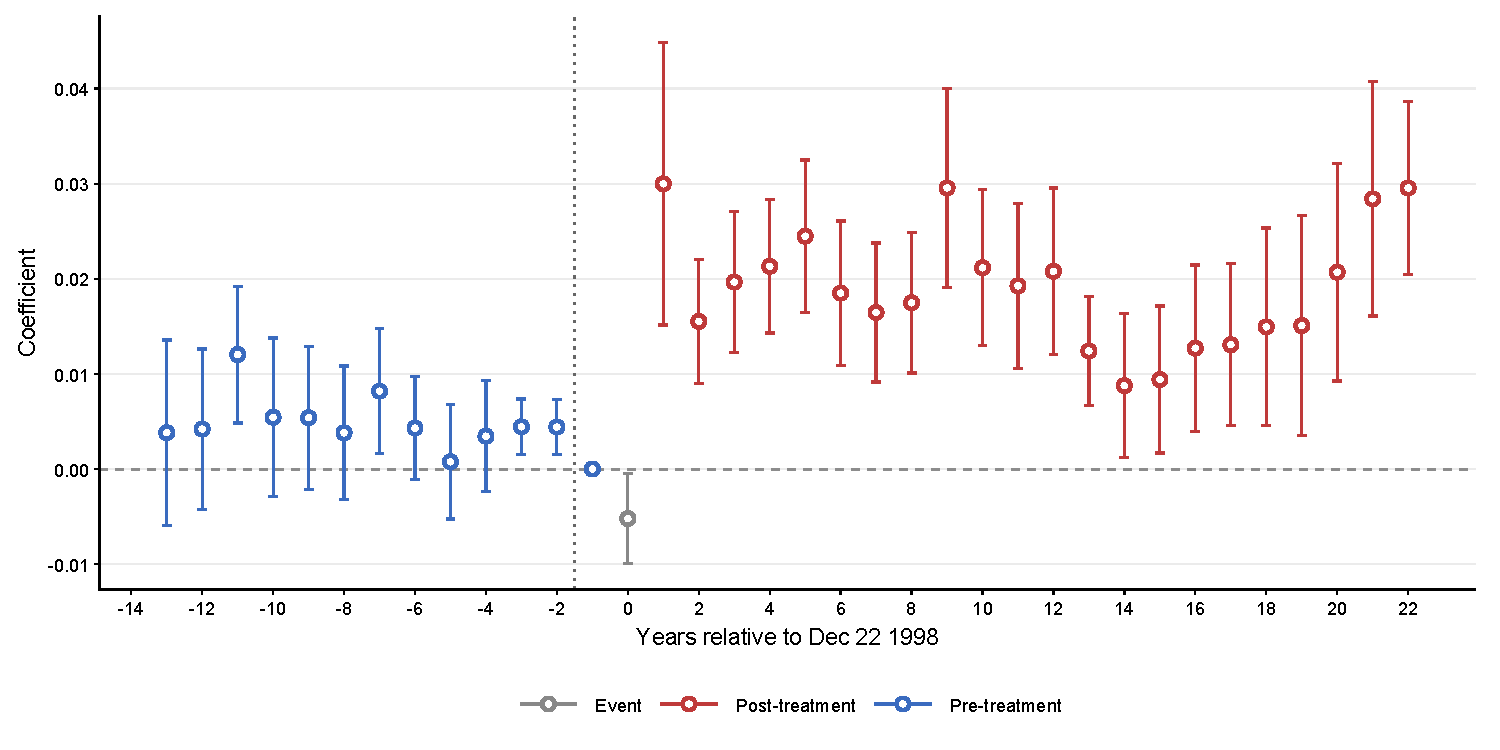
\includegraphics[height=0.78\textheight,keepaspectratio]{../../Output/Figures/Fig_ES_Full.pdf}
\end{center}
\end{frame}

\begin{frame}{Heterogeneity: Pre-89 Vintage Drives the Effect}
\phantomsection\label{heterogeneity-pre-89-vintage-drives-the-effect}
\BerkeleyLightMode

\vspace{0.15cm}
\begin{center}
\scriptsize

\begingroup
\centering
\begin{tabular}{lcccc}
   \toprule
                                            & (1) Raw        & (2) + Fac FE   & (3) + Controls & (4) + Cell FE \\   
                                            & (1)            & (2)            & (3)            & (4)\\  
   \midrule 
   Constant                                 & 0.0103$^{***}$ &                &                &   \\   
                                            & (0.0011)       &                &                &   \\   
   did\_term                                & 0.0048$^{***}$ & 0.0117$^{***}$ & 0.0114$^{***}$ & -0.0067$^{**}$\\   
                                            & (0.0011)       & (0.0028)       & (0.0029)       & (0.0031)\\   
   pre89\_cohort                            & 0.0135$^{***}$ & 0.0671$^{***}$ & 0.0696$^{***}$ &   \\   
                                            & (0.0023)       & (0.0062)       & (0.0060)       &   \\   
   did\_term $\times$ pre89\_cohort         & 0.0094$^{***}$ & 0.0382$^{***}$ & 0.0360$^{***}$ & 0.0309$^{***}$\\   
                                            & (0.0023)       & (0.0029)       & (0.0029)       & (0.0065)\\   
   mandate\_release\_det                    &                &                & -0.0114$^{**}$ &   \\   
                                            &                &                & (0.0040)       &   \\   
   mandate\_spill\_overfill                 &                &                & 0.0009         &   \\   
                                            &                &                & (0.0028)       &   \\   
   mandate\_integrity                       &                &                & 0.0044         &   \\   
                                            &                &                & (0.0030)       &   \\   
    \\
   Observations                             & 9,761,982      & 9,761,982      & 9,761,982      & 9,761,044\\  
   R$^2$                                    & 0.00249        & 0.04685        & 0.04750        & 0.07772\\  
   Within R$^2$                             &                & 0.01392        & 0.01460        & 0.00065\\  
    \\
   panel\_id fixed effects                  &                & $\checkmark$   & $\checkmark$   & $\checkmark$\\   
   cell\_vintage\_year\_fe fixed effects    &                &                &                & $\checkmark$\\   
   \bottomrule
\end{tabular}
\par\endgroup



\end{center}

\centering\small

\textit{Pre-89 ATT $= \hat\beta_0 + \hat\beta_1 \approx +3.1$ pp; post-88 ATT $= \hat\beta_0 \approx +0.6$ pp.}

\begin{tikzpicture}[remember picture, overlay]
\node[anchor=south west, inner sep=0pt] at ([xshift=10pt, yshift=10pt]current page.south west) {%
  \navbutton[vintage-forest][fill=BerkeleyBlue, font=\tiny, inner sep=2pt]{ATT by install year $\rightarrow$}%
};
\end{tikzpicture}
\end{frame}

\begin{frame}{LUST Discovery: Both Channels Fall}
\phantomsection\label{lust-discovery-both-channels-fall}
\BerkeleyLightMode

\vspace{0.15cm}
\begin{center}
\scriptsize
\begin{tabular}{lcc}
\toprule
Outcome & Pre-reform ctrl mean & TX $\times$ Post \\
\midrule
Any leak found this year                       & 1.73\% & $-$1.27\,pp\textsuperscript{***} \\
                                               &        & (0.0032)                         \\
\midrule
\multicolumn{3}{l}{\textit{By how the leak was discovered:}}                                \\
\hspace{0.5em}Routine monitoring               & 1.16\% & $-$0.76\,pp\textsuperscript{***} \\
\hspace{0.5em}\textit{(no closure in $\pm$60d)}&        & (0.0021)                         \\
\hspace{0.5em}Closure-inspection finding       & 0.61\% & $-$0.51\,pp\textsuperscript{**}  \\
\hspace{0.5em}\textit{(closure within 60d)}    &        & (0.0017)                         \\
\midrule
$N$ facility-years & \multicolumn{2}{c}{4{,}650{,}240}                                                  \\
Sample             & \multicolumn{2}{c}{Incumbent (alive at Dec 22, 1998)}                             \\
FE                 & \multicolumn{2}{c}{Facility + cell $\times$ year; cluster by state}    \\
\bottomrule
\end{tabular}

\end{center}

\begin{tikzpicture}[remember picture, overlay]
\node[anchor=south west, inner sep=0pt] at ([xshift=10pt, yshift=10pt]current page.south west) {%
  \navbutton[lust-es][fill=BerkeleyBlue, font=\tiny, inner sep=2pt]{LUST event study $\rightarrow$}%
};
\end{tikzpicture}
\end{frame}

\begin{frame}{What Closing Firms Do: Composition Shifts to Replacement}
\phantomsection\label{what-closing-firms-do-composition-shifts-to-replacement}
\BerkeleyLightMode

\vspace{0.1cm}
\begin{center}
\scriptsize
\small
\begin{tabular}{lcc}
\toprule
Outcome (conditional on closing) & Pre-reform ctrl mean & TX $\times$ Post \\
\midrule
Facility closes all tanks this year     & 70.9\%       & $+$6.5\,pp\textsuperscript{***} \\
                                        &              & (0.019)                          \\
Has a permanent closure (no replace)    & 88.3\%       & $-$6.2\,pp\textsuperscript{***} \\
                                        &              & (0.012)                          \\
Has a replacement closure (upgrade)     & 12.0\%       & $+$6.3\,pp\textsuperscript{***} \\
                                        &              & (0.013)                          \\
Any DW tank installed                   & 4.1\%        & $-$1.4\,pp\textsuperscript{*}   \\
                                        &              & (0.007)                          \\
Net tank change (count)                 & $-$1.905     & $+$0.020                         \\
                                        &              & (0.085)                          \\
Capacity change (gal)                   & $-$100{,}394 & $-$1{,}397                       \\
                                        &              & (5{,}715)                        \\
\midrule
$N$ closing facility-years & \multicolumn{2}{c}{59{,}107}                                                       \\
Sample                     & \multicolumn{2}{c}{Incumbent, any\_closure $=1$}                                   \\
FE                         & \multicolumn{2}{c}{Facility + make\_model\_fac $\times$ year; cluster by state}    \\
\bottomrule
\end{tabular}

\end{center}

\centering\small

\textit{Conditional on closing (sample is endogenous). Headline: replacement margin nearly doubles ($+53\%$ relative); aggregate exit volume flat.}
\end{frame}

\begin{frame}{}
\phantomsection\label{section-3}
\BerkeleyMode

\begin{center}
\Huge \textbf{Structural Model}
\end{center}
\end{frame}

\begin{frame}{Model Setup}
\phantomsection\label{model-setup}
\BerkeleyLightMode

\textbf{State.} \(s_t = (a_t, W_i, R_i, \varepsilon_t)\) --- 9 age bins
\(\times\) 2 wall types \(\times\) 2 regimes \(= 36\) states. Actions:
maintain / exit / replace.

\textbf{Flow utility} (annual net revenue \(R\) normalized to 1;
\emph{not directly observed} --- the model identifies \(\theta\) in
units of \(R\)).

\begin{align*}
u^m(s) &= 1 - \gamma_p\, p_t - \gamma_r\, h(a_t)\, L \\
u^e(s) &= \kappa \quad \text{(scrap value)} \\
u^r(s) &= -K \quad \text{(install new DW tank)}
\end{align*}

\textbf{Calibrated upstream} \emph{(outside the model)}: premium
\(p_t\), hazard \(h(a_t)\), liability \(L\) --- all from the
descriptive-evidence section.

\textbf{Estimated jointly} \emph{(inside the model)}:
\(\theta = (\kappa, K, \gamma_p, \gamma_r)\). NPL match of choice shares
across \((a, W, R)\) cells.
\end{frame}

\begin{frame}{Identification}
\phantomsection\label{identification}
\BerkeleyLightMode

Each parameter is identified by a distinct moment in the choice data:

\begin{itemize}
\tightlist
\item
  \(\kappa\): the unconditional exit rate \(P(\text{exit} \mid s)\)
\item
  \(K\): the replace-vs-exit share among closing tanks
\item
  \(\gamma_p\): cross-cell response of choice shares to premium
  variation in \((a, W, R)\)
\item
  \(\gamma_r\): divergence in age-closure hazard between uniform-premium
  and risk-based regimes
\end{itemize}

NPL (Aguirregabiria \& Mira 2007); AM-2002 profile-likelihood SEs.
\end{frame}

\begin{frame}{Structural Estimating Sample}
\phantomsection\label{structural-estimating-sample}
\BerkeleyLightMode

\textbf{Unit of observation.} Facility-year. One row per facility per
year, 1999--2018.

\textbf{Sample.} Texas facilities, post-reform period. The structural
model fits the \emph{equilibrium} of the risk-based regime --- TX is the
regime that's actually priced.

\begin{itemize}
\tightlist
\item
  Roughly 26k TX incumbent facilities over 20 years \(\approx\) 520k
  facility-years
\item
  After dropping rows with missing premium or hazard inputs: \(\approx\)
  430k facility-years
\item
  Choices observed: maintain / exit / replace; mapped onto 32 state
  cells \((a, W, R)\)
\item
  Premiums \(p_t\) from Mid-Continent rate-filing reconstruction;
  hazards \(h(a_t)\) from the first-release-prediction model
\end{itemize}
\end{frame}

\begin{frame}{Parameter Estimates}
\phantomsection\label{parameter-estimates}
\BerkeleyLightMode

\vspace{0.3cm}
\begin{center}
% Auto-generated by 04f_Replacement_Refit_Extended2000_AM_SE.R
% AM (2002) corrected SEs in (parentheses); bootstrap SEs deferred.
\begin{tabular}{lcc}
\hline
 & Observed & Extended (2000+) \\
 & TX 2006+, controls 1999+ & TX 2000+, controls 2000+ \\
\hline
$\kappa_{\mathrm{exit}}$ (\$) & \$261,222 & \$257,702 \\
        & (\$306) & (\$310) \\
$K$ (\$) & \$51,779 & \$52,658 \\
        & (\$142) & (\$146) \\
$\gamma_{\mathrm{price}}$ & -0.293 & -1.142 \\
        & (0.049) & (0.048) \\
$\gamma_{\mathrm{risk}}$ & 0.164 & 0.153 \\
        & (0.003) & (0.003) \\
\hline
$\log L$ & -268,481 & -247,614 \\
$N$ obs  & 2,282,735 & 2,300,780 \\
\hline
\multicolumn{3}{l}{\footnotesize SEs are AM (2002) profile-likelihood;
  bootstrap SEs deferred for a future pass.}
\end{tabular}

\end{center}
\end{frame}

\begin{frame}{Estimates in Economic Terms}
\phantomsection\label{estimates-in-economic-terms}
\BerkeleyLightMode

\textit{Reminder: all parameters are in units of annual net revenue $R$. Dollar translations below use a calibration anchor of $R \approx \$10$k/yr per facility }

\begin{itemize}
\item
  \textbf{\(\hat\kappa \approx 26\,R\)} (about \$261k under the
  calibration). Net scrap value when a facility exits; large in absolute
  terms, consistent with land-value liquidation net of remediation
  liability.
\item
  \textbf{\(\hat K \approx 5\,R\)} (about \$52k). Replacement cost for a
  new double-walled tank; in line with industry estimates.
\item
  \textbf{\(\hat\gamma_p = -0.29\).} a one-unit (\(\approx 1\,R\))
  increase in premium reduces the maintain-flow value by 0.29 units.
\item
  \textbf{\(\hat\gamma_r = 0.16\).} The point estimate is small relative
  to a fully-internalized benchmark (\(\gamma_r = 1\)).
\end{itemize}
\end{frame}

\begin{frame}{Counterfactual Policy Scenarios}
\phantomsection\label{counterfactual-policy-scenarios}
\BerkeleyLightMode

\begin{longtable}[]{@{}
  >{\raggedright\arraybackslash}p{(\columnwidth - 2\tabcolsep) * \real{0.5000}}
  >{\raggedright\arraybackslash}p{(\columnwidth - 2\tabcolsep) * \real{0.5000}}@{}}
\toprule\noalign{}
\begin{minipage}[b]{\linewidth}\raggedright
Policy
\end{minipage} & \begin{minipage}[b]{\linewidth}\raggedright
Mechanism
\end{minipage} \\
\midrule\noalign{}
\endhead
\textbf{Subsidy} & \(K \to 0.5\, K\) --- replacement cost halved \\
\textbf{Pigouvian} & Add \(h(a)\cdot E\) to maintain cost;
\(E = \$17{,}000\) (Marcus, 2021) \\
\textbf{Mandate} & Force \(P(\text{maintain}) = 0\) for \(a \geq 6\)
(age 25+) \\
\bottomrule\noalign{}
\end{longtable}

\textbf{What we do for each policy.} Recompute firms' optimal choices
under the new price/cost regime, let the fleet settle into its long-run
age-and-wall distribution, then add up the present-value impact on three
groups: firms (operating profits), the environment (avoided cleanup and
health damages), and the government (subsidies paid out).
\end{frame}

\begin{frame}{Welfare Decomposition}
\phantomsection\label{welfare-decomposition}
\BerkeleyLightMode

\vspace{0.2cm}
\begin{center}
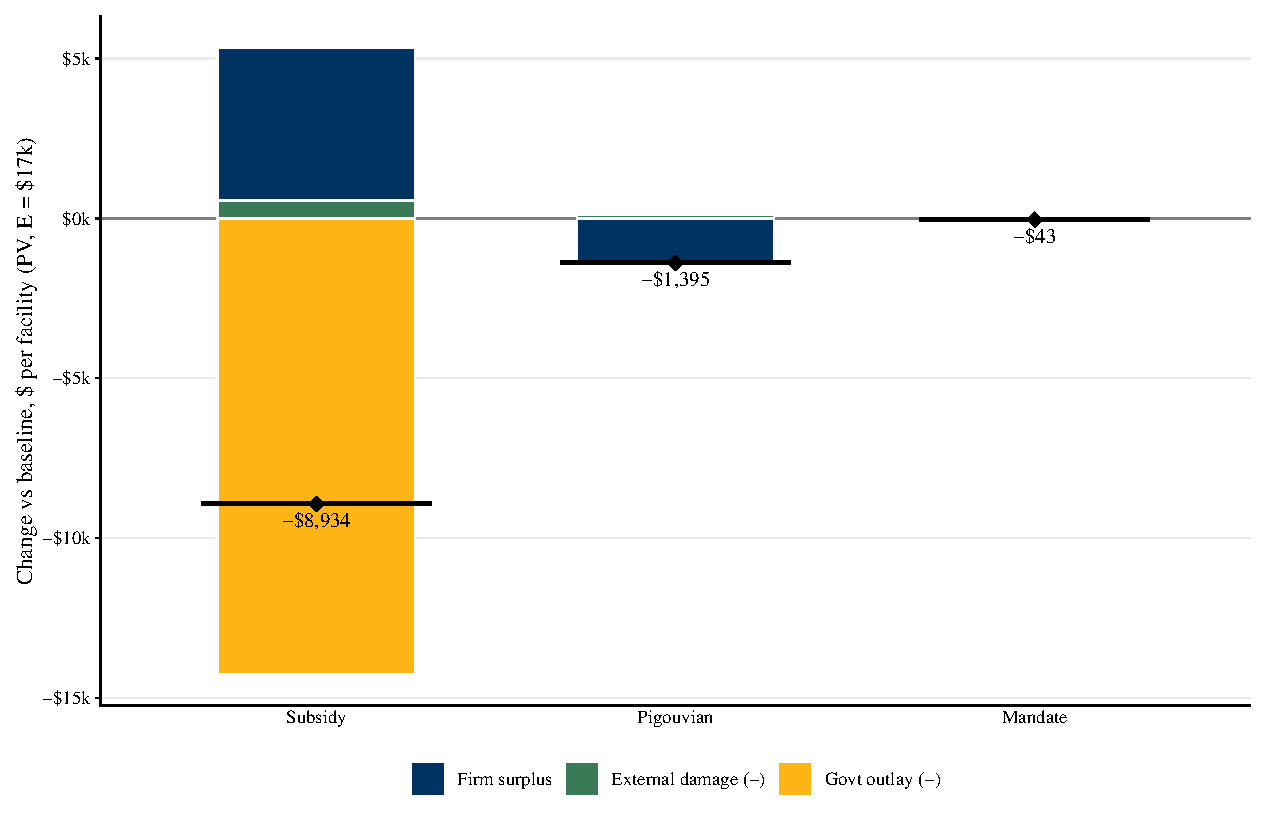
\includegraphics[height=0.78\textheight,keepaspectratio]{../../Output/Figures/04j_4p_Welfare_BarChart.pdf}
\end{center}
\end{frame}

\begin{frame}{Counterfactual Welfare Summary}
\phantomsection\label{counterfactual-welfare-summary}
\BerkeleyLightMode

\vspace{0.4cm}
\begin{center}
\begin{tabular}{lcccccc}
\toprule
 & $\bar P(M)$ & $\bar P(E)$ & $\bar P(R)$ & Firm Surplus & Social Welfare & $\Delta W$ \\
\midrule
Baseline & 98.0\% & 1.7\% & 0.2\% & \$307,724 & \$305,344 & $\pm$\$0 \\
Subsidy & 96.2\% & 1.1\% & 2.8\% & \$312,498 & \$296,409 & $-$\$8,934 \\
Pigouvian & 97.7\% & 2.0\% & 0.2\% & \$306,225 & \$303,948 & $-$\$1,395 \\
Mandate & 98.0\% & 1.8\% & 0.2\% & \$307,633 & \$305,301 & $-$\$43 \\
\bottomrule
\end{tabular}

\end{center}

\vfill

\centering

\textit{All three CFs reduce social welfare at $E = \$17$k. Subsidy hurts most: govt outlay outweighs firm-surplus gain. Mandate roughly neutral.}
\end{frame}

\begin{frame}{Takeaways}
\phantomsection\label{takeaways}
\BerkeleyLightMode

\begin{enumerate}
\item
  \textbf{Risk-based pricing does shift behavior.} A \(+1.58\) pp annual
  closure ATT --- about \(4\times\) larger in the pre-1989 SW-heavy
  stock that the schedule actually prices.
\item
  \textbf{The shift is on the composition margin, not exit volume.}
  Conditional on closing, the \textbf{replacement} rate nearly doubles
  (\(12\% \to 18\%\)); net tank counts and capacity barely move. LUST
  discovery falls through both background and inspection-triggered
  channels.
\item
  \textbf{Welfare under the priced regime is still below first-best.}
  All three counterfactual policies --- \(K\) subsidy, Pigouvian
  surcharge on \(h(a)\cdot E\), age-25 mandate --- \emph{reduce} social
  welfare at \(E = \$17\)k. RBP is a partial fix; closing the residual
  wedge requires direct intervention beyond the actuarial price signal.
\end{enumerate}
\end{frame}

\begin{frame}{Appendix: ATT by Installation Vintage}
\phantomsection\label{appendix-att-by-installation-vintage}
\BerkeleyLightMode

\hypertarget{vintage-forest}{}

\vspace{0.2cm}
\begin{center}
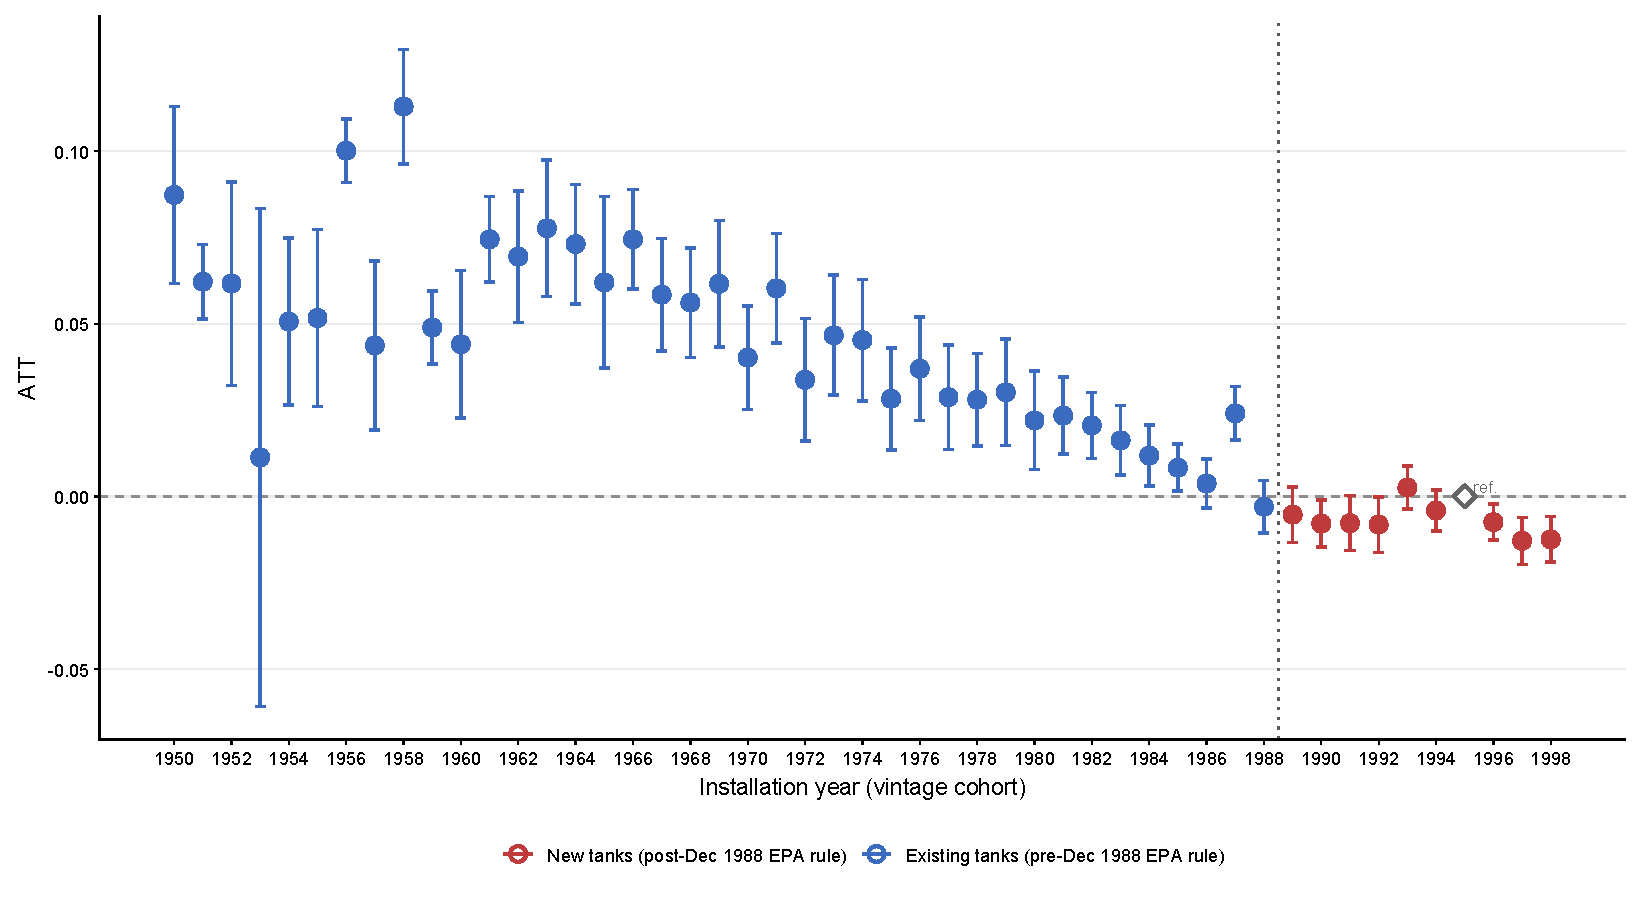
\includegraphics[height=0.78\textheight,keepaspectratio]{../../Output/Figures/Fig_Vintage_Forest.pdf}
\end{center}
\end{frame}

\begin{frame}{Appendix: Cell-Level Goodness of Fit}
\phantomsection\label{appendix-cell-level-goodness-of-fit}
\BerkeleyLightMode

\hypertarget{cell-gof}{}

\vspace{0.2cm}
\begin{center}
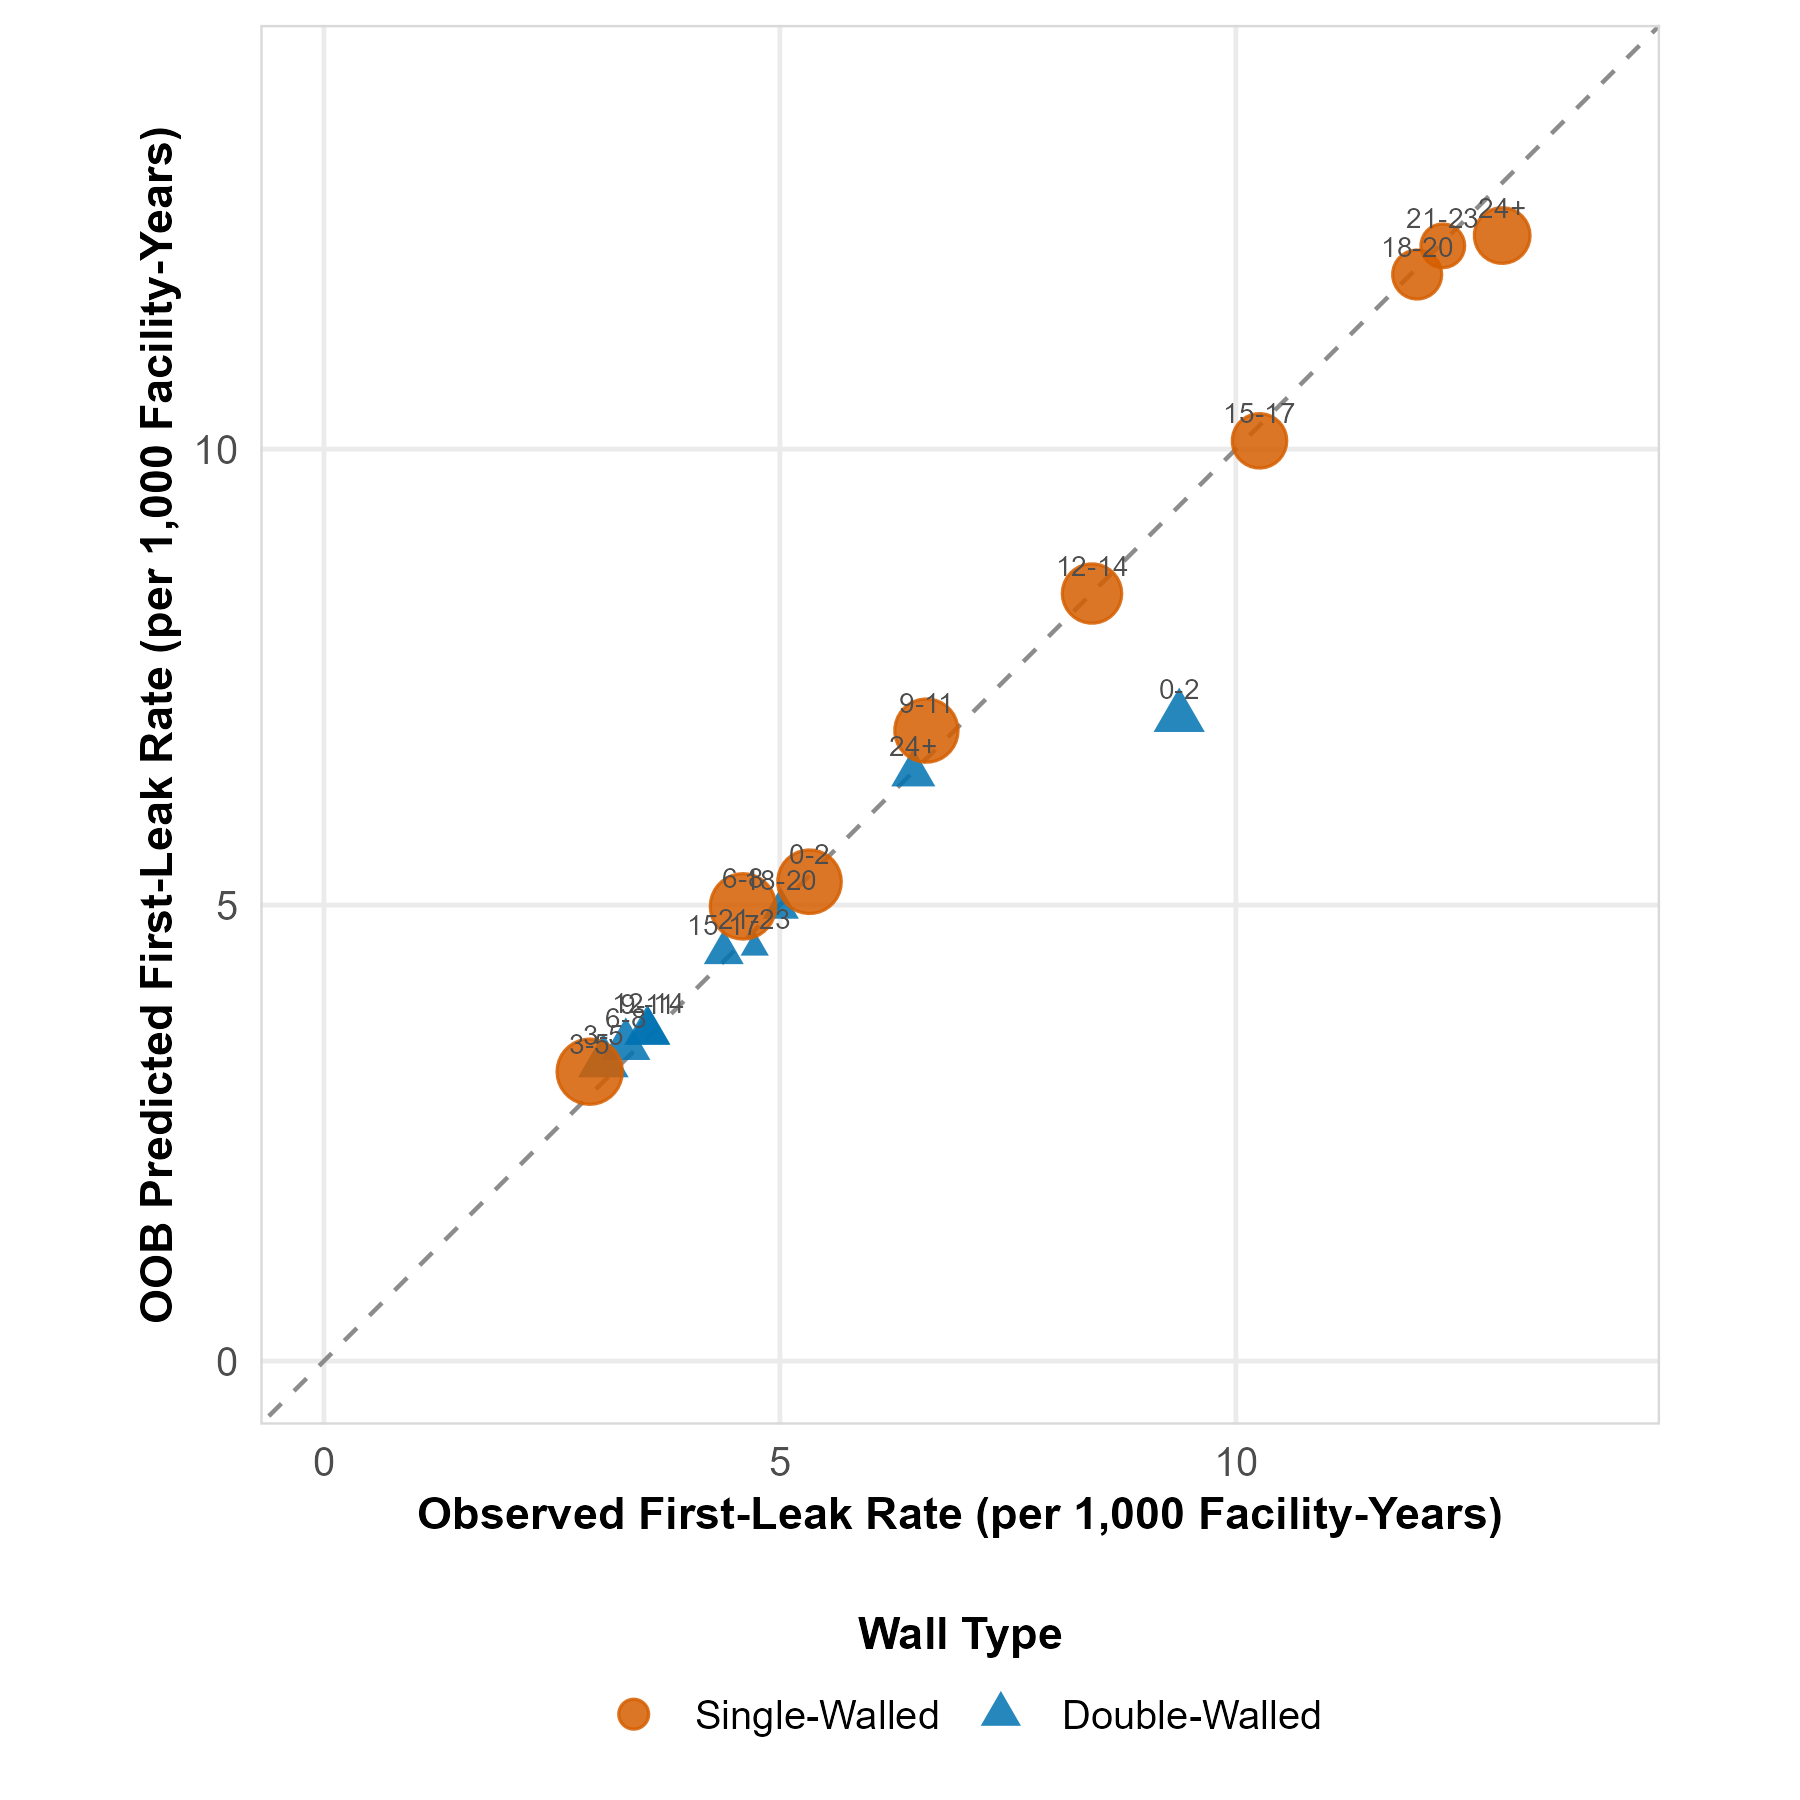
\includegraphics[height=0.78\textheight,keepaspectratio]{../../Output/Figures/Figure_CV_CellRisk_GoF.png}
\end{center}
\end{frame}

\begin{frame}{Appendix: Premium vs.~Per-Tank Expected Loss}
\phantomsection\label{appendix-premium-vs.-per-tank-expected-loss}
\BerkeleyLightMode

\hypertarget{premium-vs-el}{}

\vspace{0.2cm}
\begin{center}
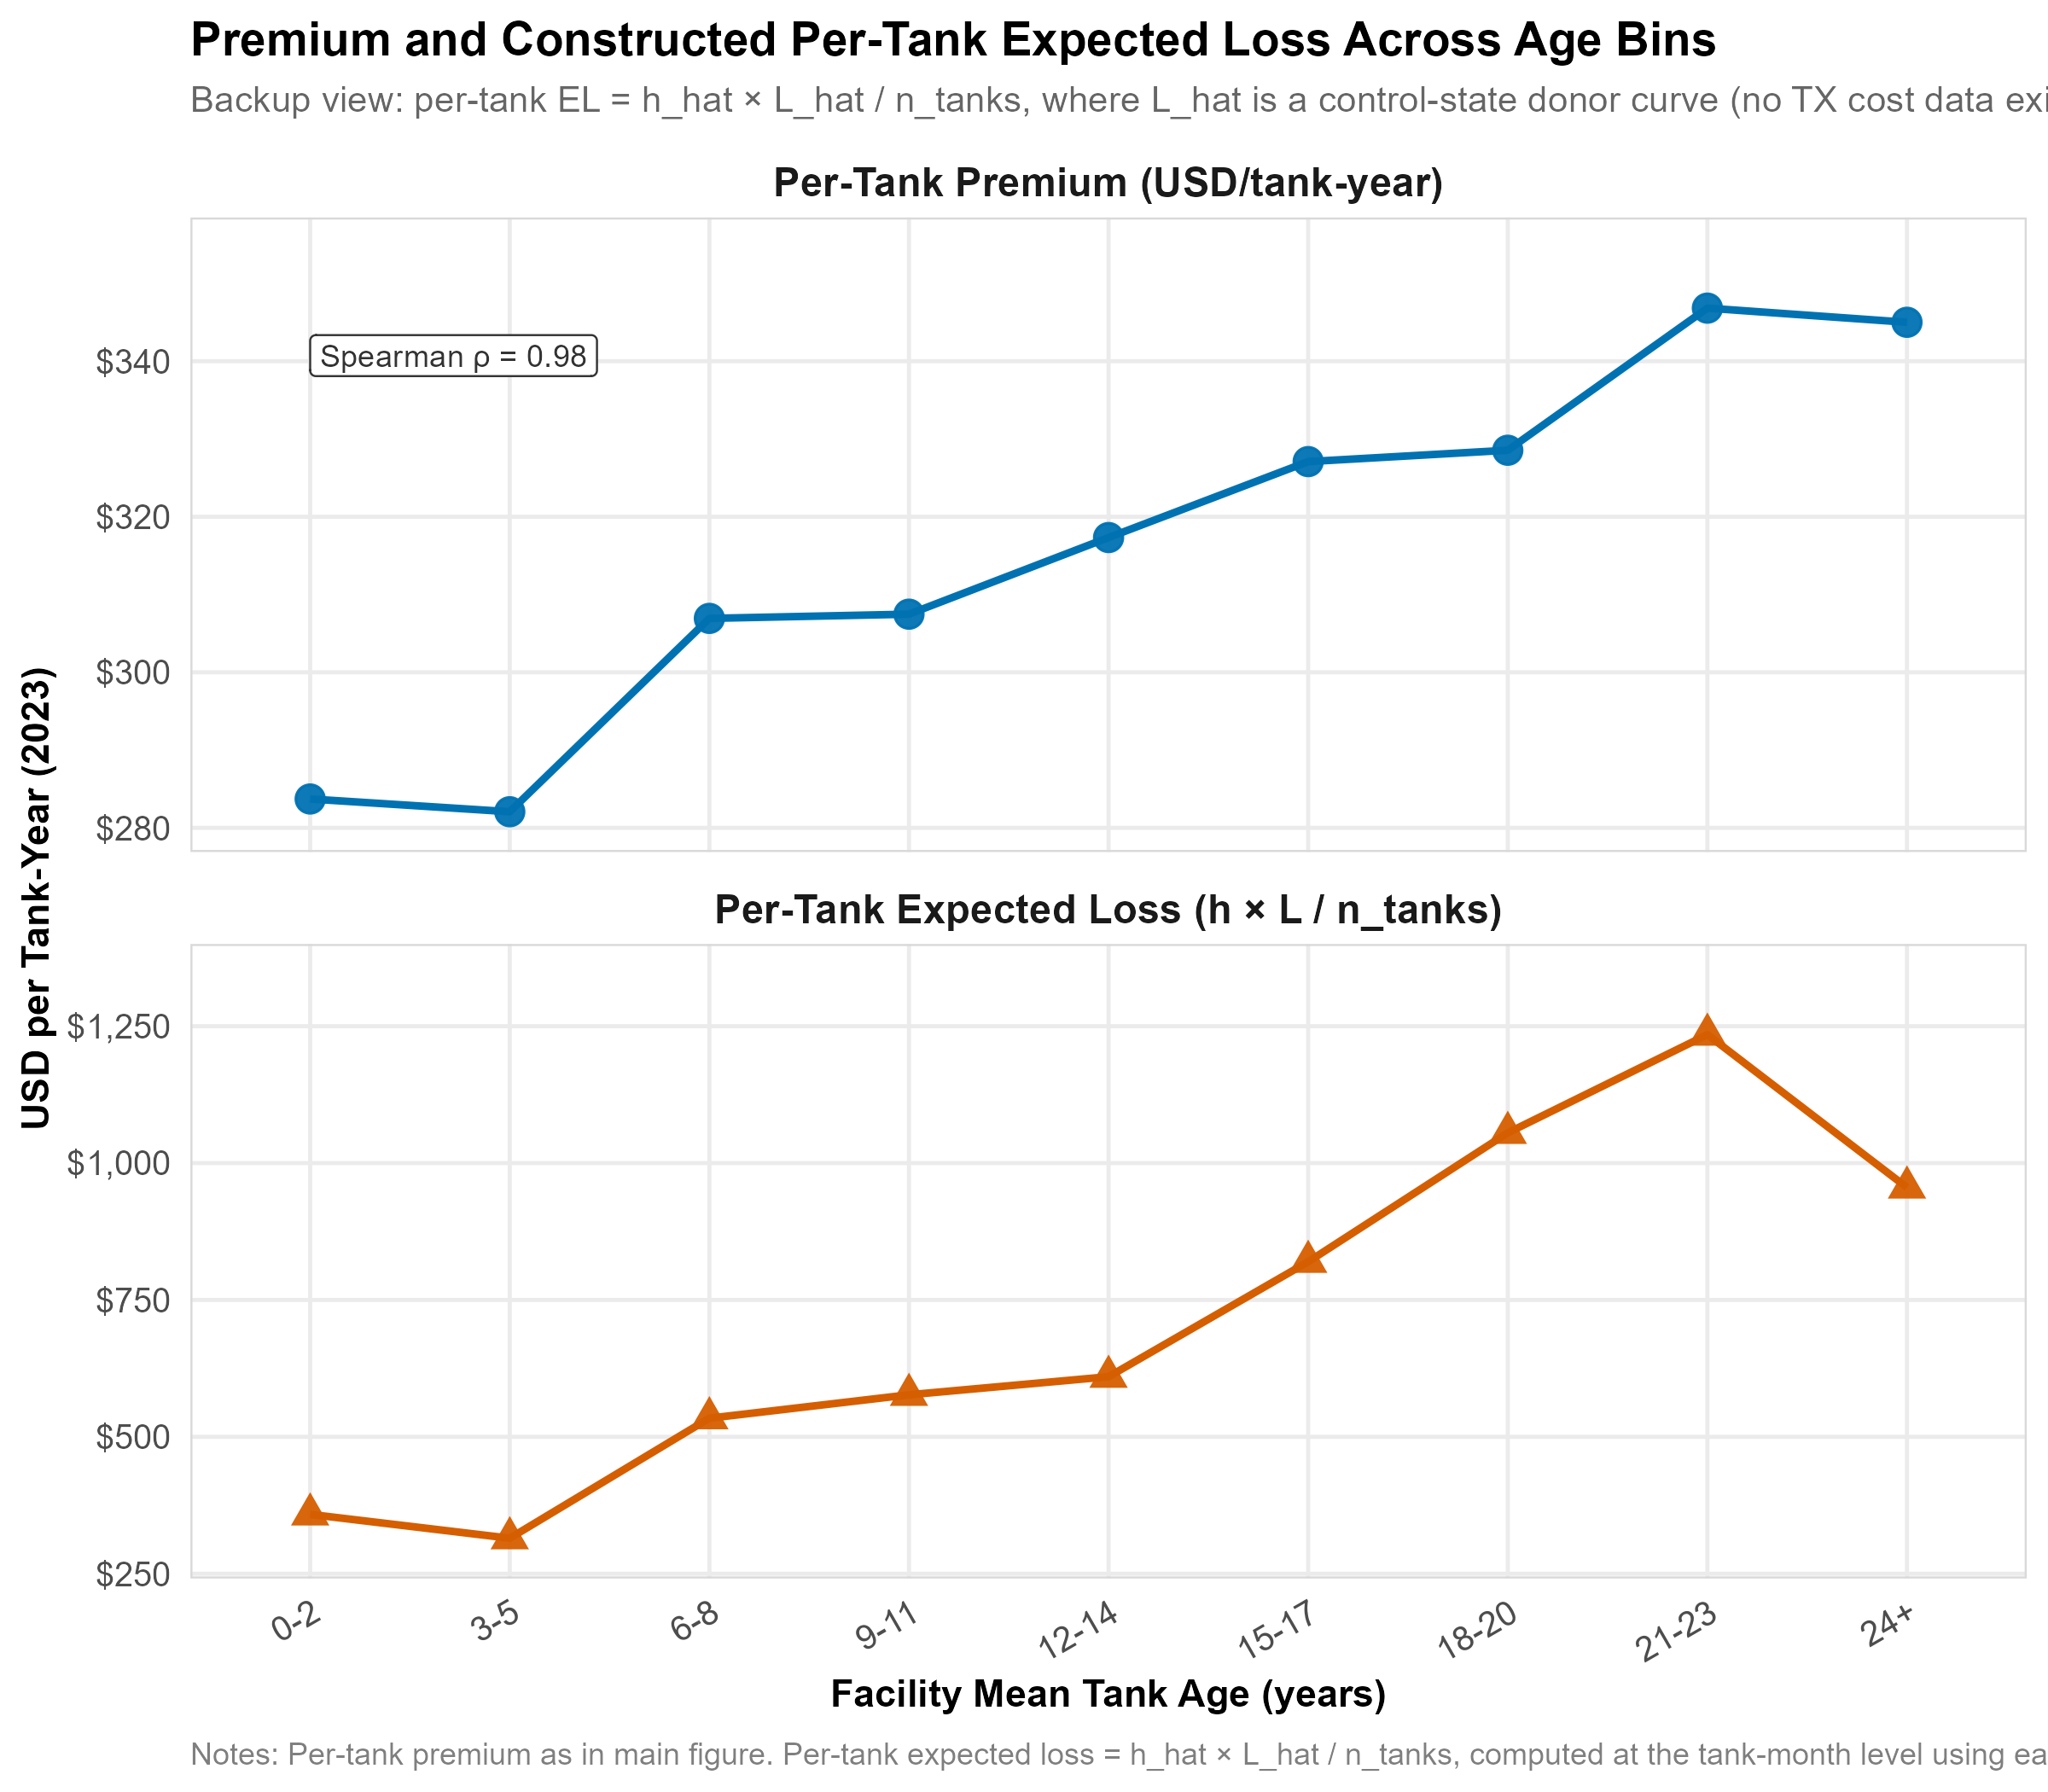
\includegraphics[height=0.78\textheight,keepaspectratio]{../../Output/Figures/Figure_Premium_vs_EL_Raw.png}
\end{center}
\end{frame}

\begin{frame}{Appendix: LUST Event Study --- Total Leak Discovery}
\phantomsection\label{appendix-lust-event-study-total-leak-discovery}
\BerkeleyLightMode

\hypertarget{lust-es}{}

\vspace{0.2cm}
\begin{center}
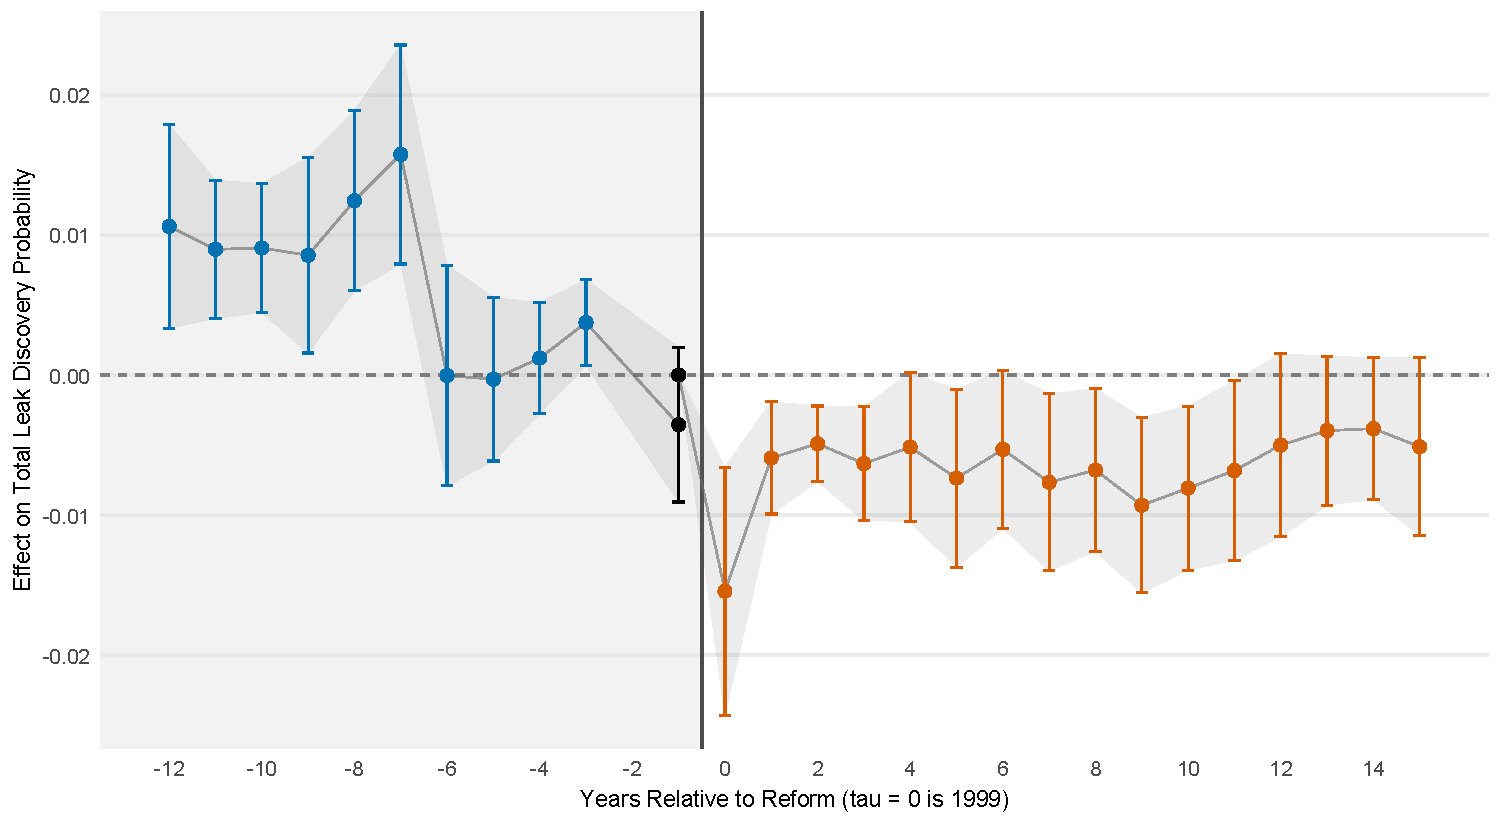
\includegraphics[height=0.78\textheight,keepaspectratio]{../../Output/Figures/Figure_ES_LUSTTotal_Appendix.pdf}
\end{center}
\end{frame}

\begin{frame}{Appendix: Subsidy Curve}
\phantomsection\label{appendix-subsidy-curve}
\BerkeleyLightMode

\vspace{0.2cm}
\begin{center}
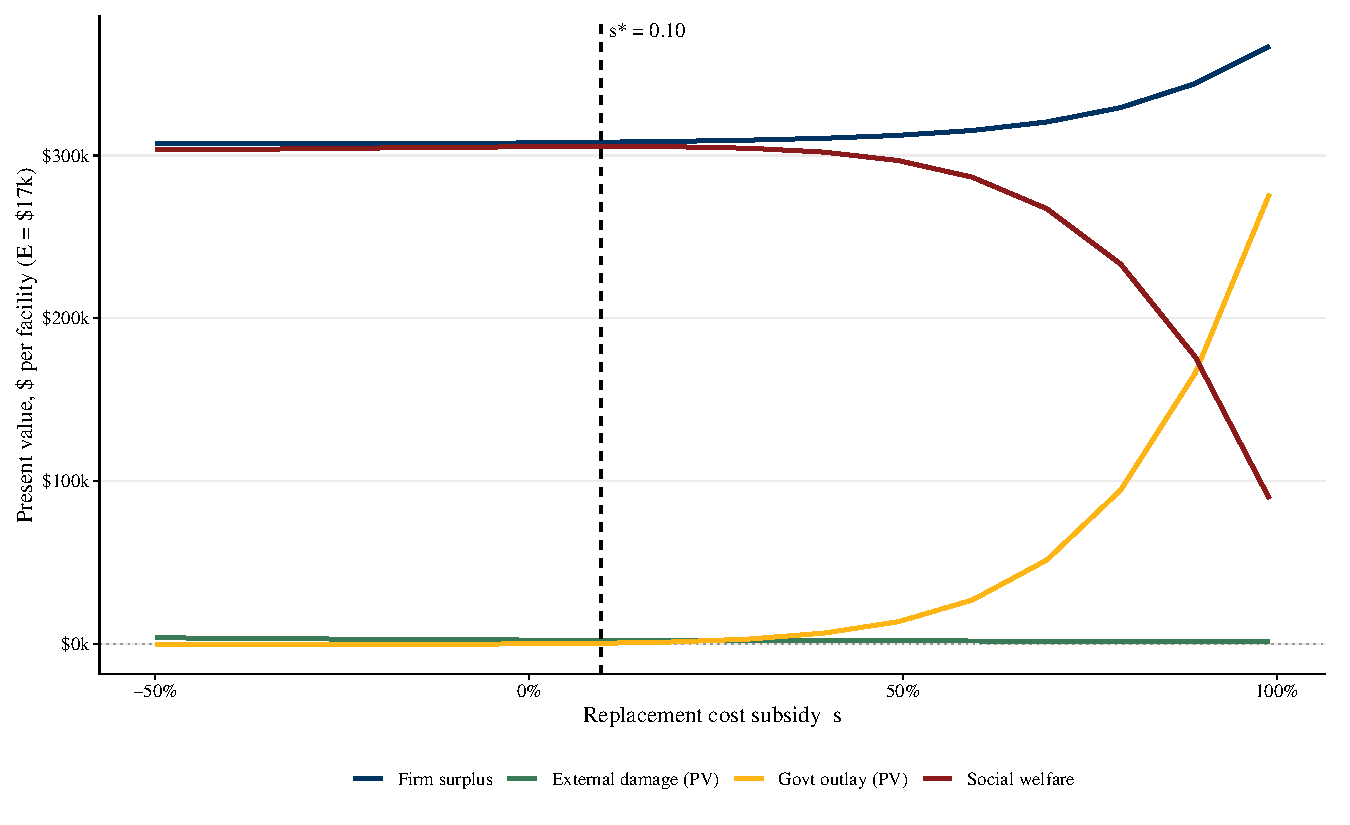
\includegraphics[height=0.78\textheight,keepaspectratio]{../../Output/Figures/04j_4p_Subsidy_Curve.pdf}
\end{center}
\end{frame}

\end{document}
